\chapter{Evaluation}\label{chap:evaluation}

\section{Stylized 3D Gaussian Splatting Avatar Creation}

To create a variety of stylized 3D Gaussian Splatting avatars, four volunteers (one shown in the previous chapter) participated in individual photoshoot sessions within the Photodome, where their images were captured. Following data capture, data preparation and initial 3D Gaussian Splatting were performed according to the steps outlined in the previous chapter, specifically in Sections \ref{sec:acquisition} to \ref{sec:3dgs_initial}. These four volunteers will be referred to as participants A, B, C, and D. The initial 3D Gaussian Splatting avatars of these participants are shown in Figure \ref{fig:igs2gs_init_participants}.


\begin{figure}[!ht]
    \centering
	\begin{subfigure}{0.12\linewidth}
        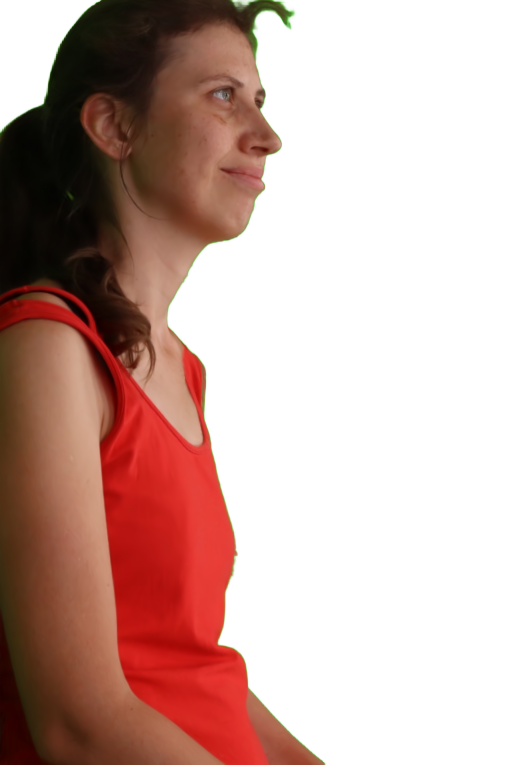
\includegraphics[width=\textwidth]{Figures/results/initials/dora/20_render.png}
        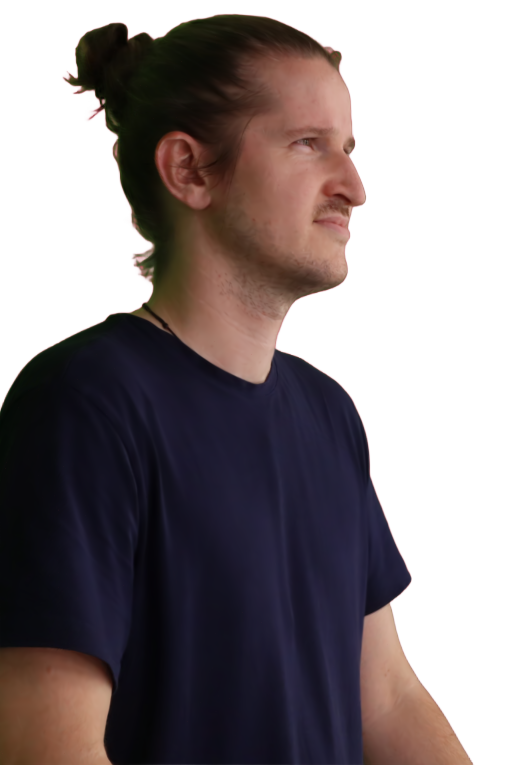
\includegraphics[width=\textwidth]{Figures/results/initials/ephra/20_render.png}
        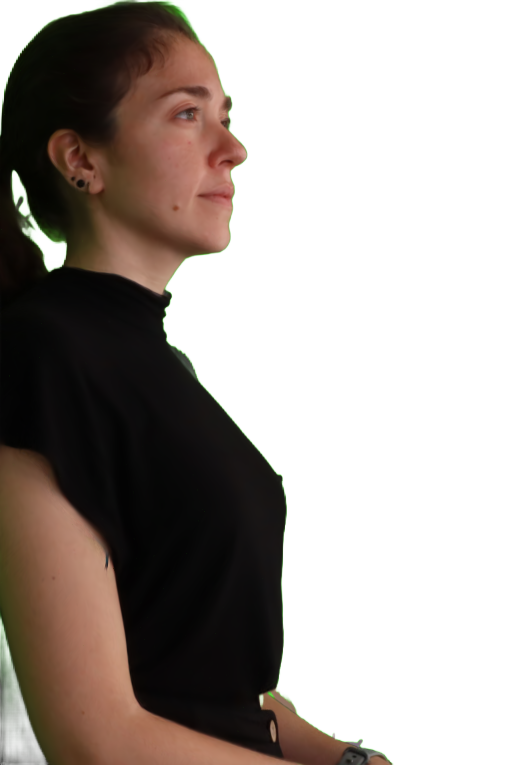
\includegraphics[width=\textwidth]{Figures/results/initials/irene/20_render.png}
        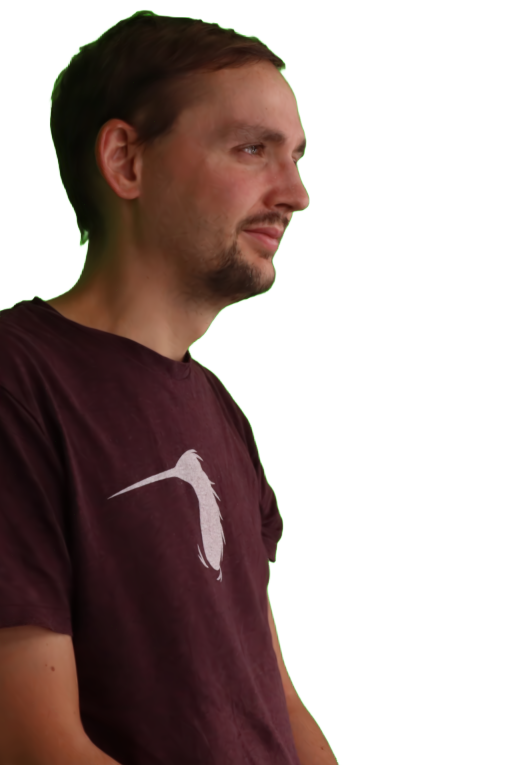
\includegraphics[width=\textwidth]{Figures/results/initials/simon/20_render.png}
	\end{subfigure}
    \begin{subfigure}{0.12\linewidth}
        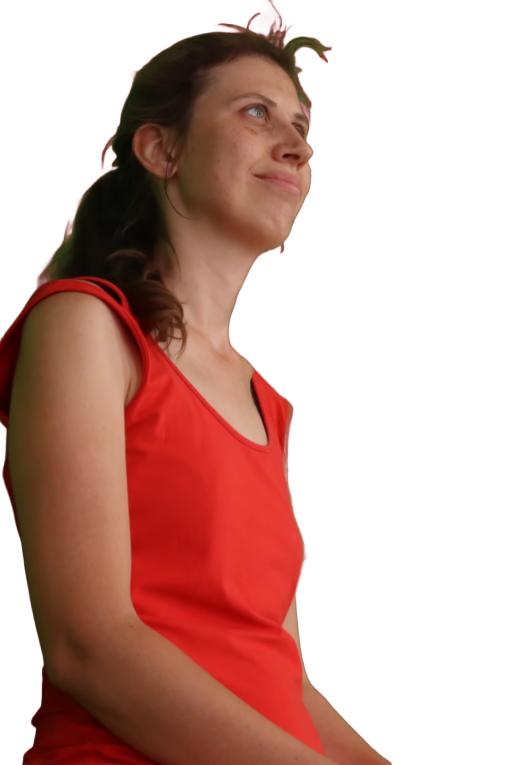
\includegraphics[width=\textwidth]{Figures/results/initials/dora/21_render.png}
        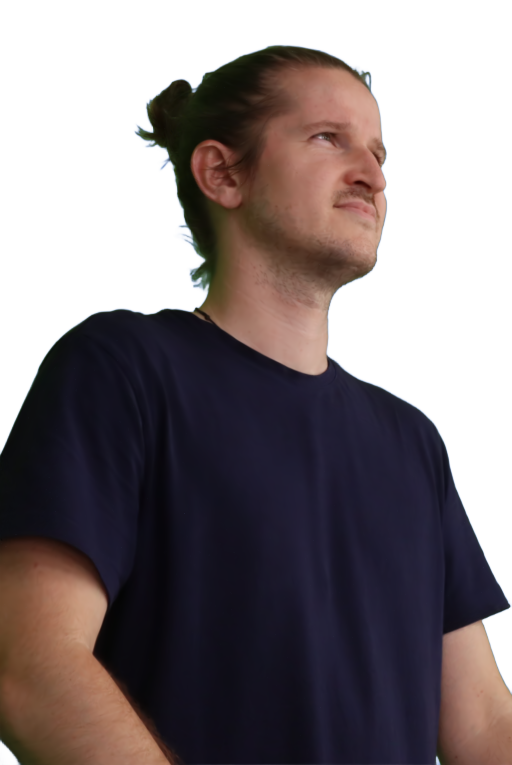
\includegraphics[width=\textwidth]{Figures/results/initials/ephra/21_render.png}
        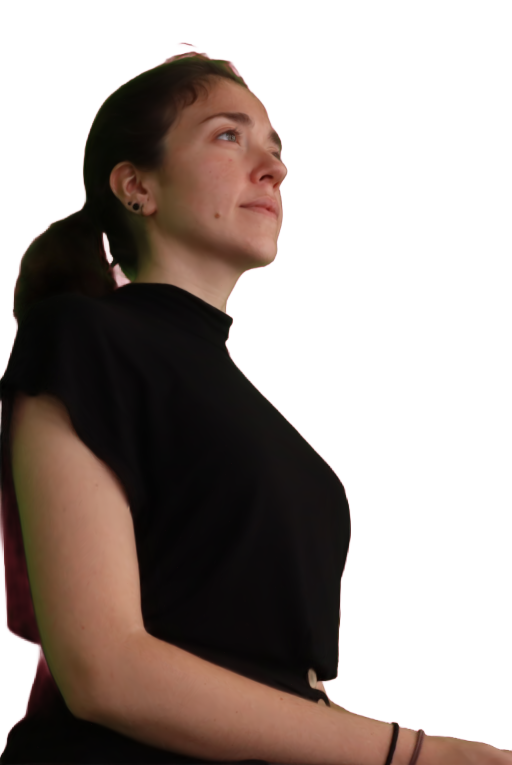
\includegraphics[width=\textwidth]{Figures/results/initials/irene/21_render.png}
        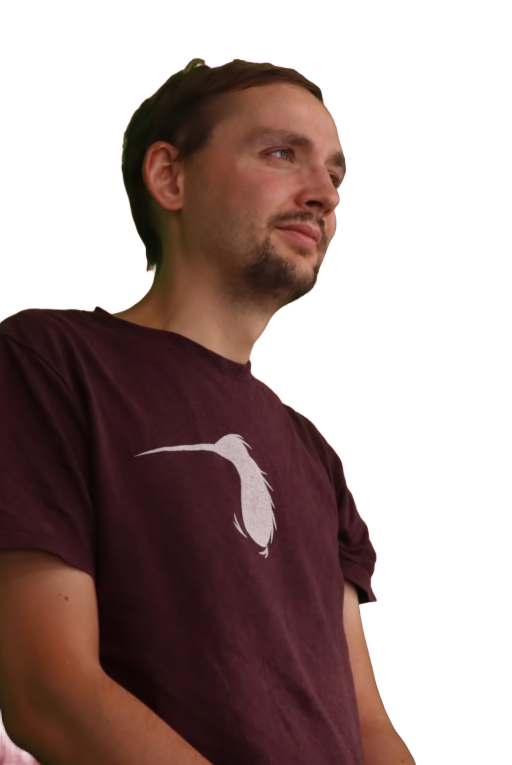
\includegraphics[width=\textwidth]{Figures/results/initials/simon/21_render.png}
	\end{subfigure}
    \begin{subfigure}{0.12\linewidth}
        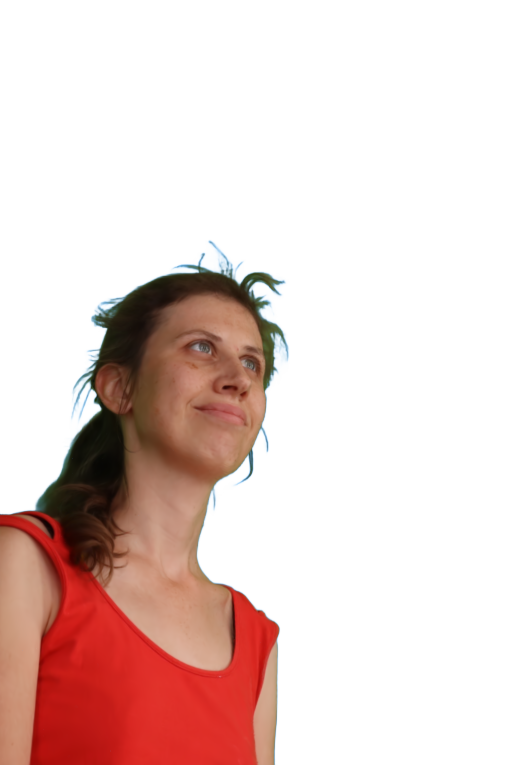
\includegraphics[width=\textwidth]{Figures/results/initials/dora/14_render.png}
        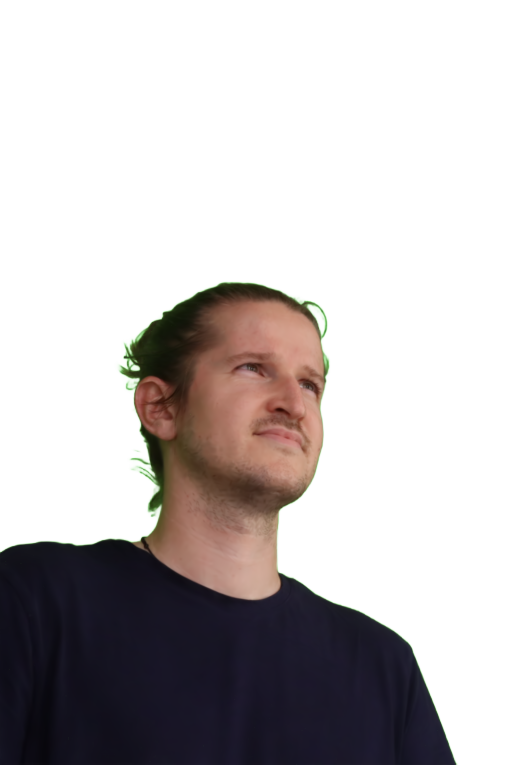
\includegraphics[width=\textwidth]{Figures/results/initials/ephra/14_render.png}
        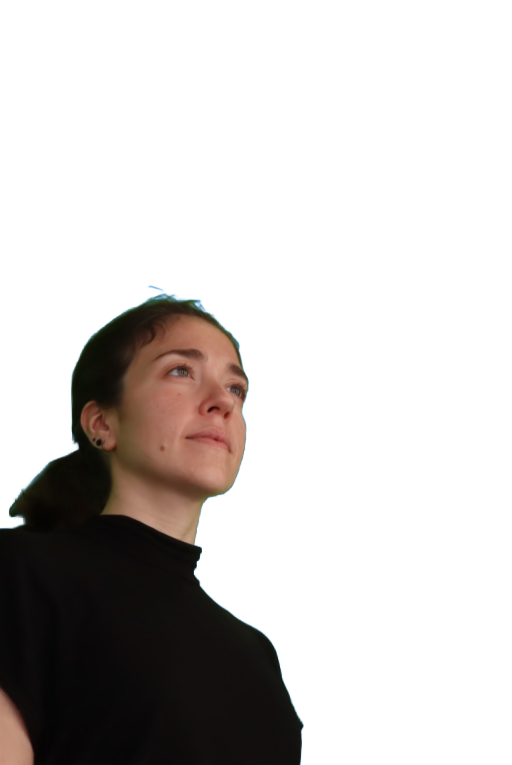
\includegraphics[width=\textwidth]{Figures/results/initials/irene/14_render.png}
        
\includegraphics[width=\textwidth]{Figures/results/initials/simon/14_render.png}
	\end{subfigure}
    \begin{subfigure}{0.12\linewidth}
        
\includegraphics[width=\textwidth]{Figures/results/initials/dora/3_render.png}
        
\includegraphics[width=\textwidth]{Figures/results/initials/ephra/3_render.png}
        
\includegraphics[width=\textwidth]{Figures/results/initials/irene/3_render.png}
        
\includegraphics[width=\textwidth]{Figures/results/initials/simon/3_render.png}
	\end{subfigure}
	\begin{subfigure}{0.12\linewidth}
        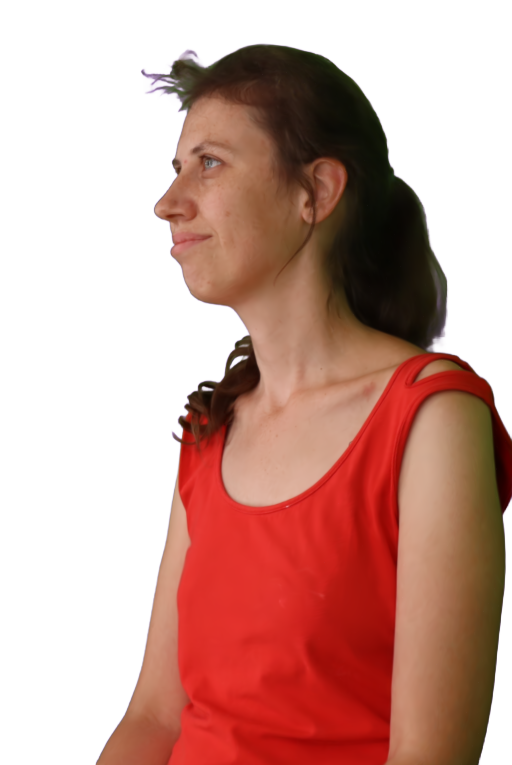
\includegraphics[width=\textwidth]{Figures/results/initials/dora/26_render.png}
        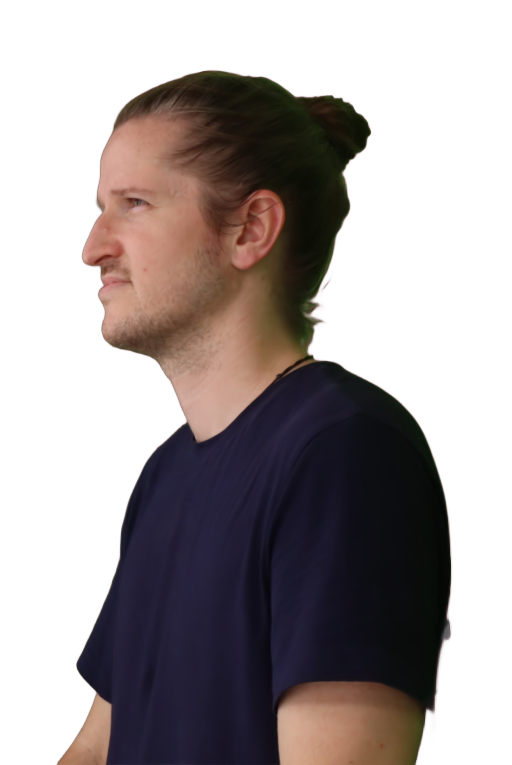
\includegraphics[width=\textwidth]{Figures/results/initials/ephra/26_render.png}
        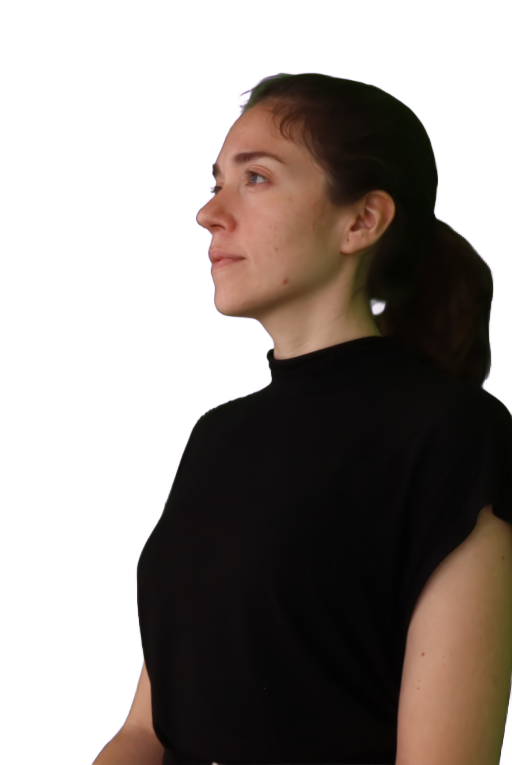
\includegraphics[width=\textwidth]{Figures/results/initials/irene/26_render.png}
        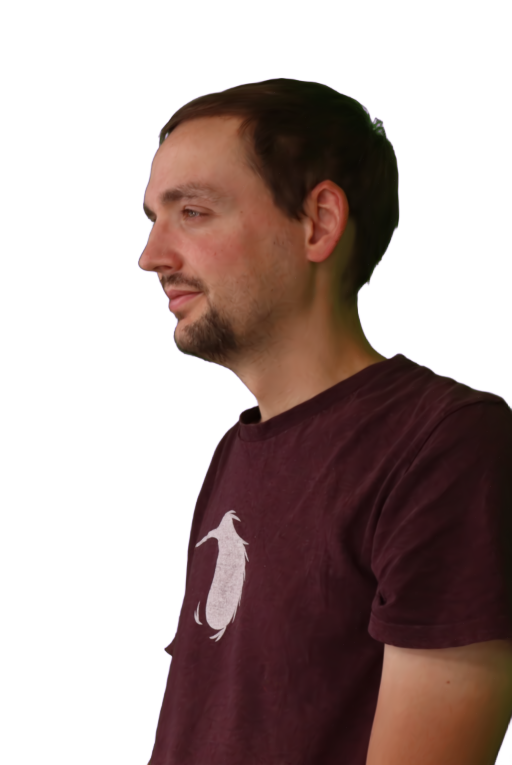
\includegraphics[width=\textwidth]{Figures/results/initials/simon/26_render.png}
	\end{subfigure}
    \begin{subfigure}{0.12\linewidth}
        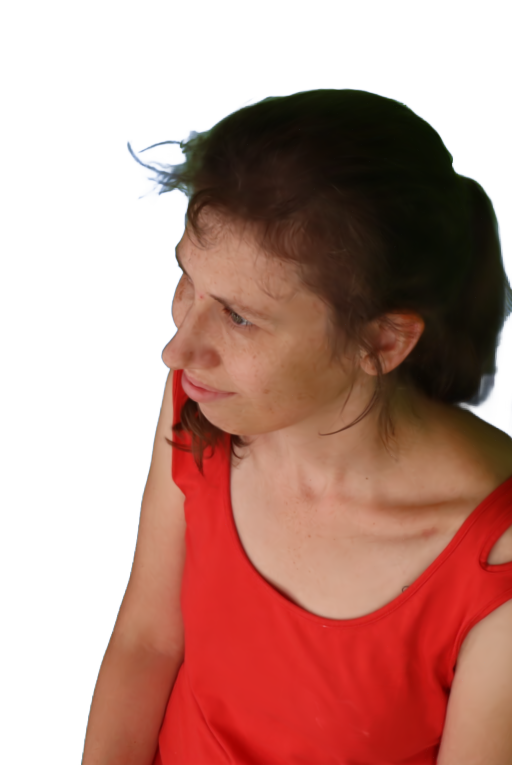
\includegraphics[width=\textwidth]{Figures/results/initials/dora/22_render.png}
        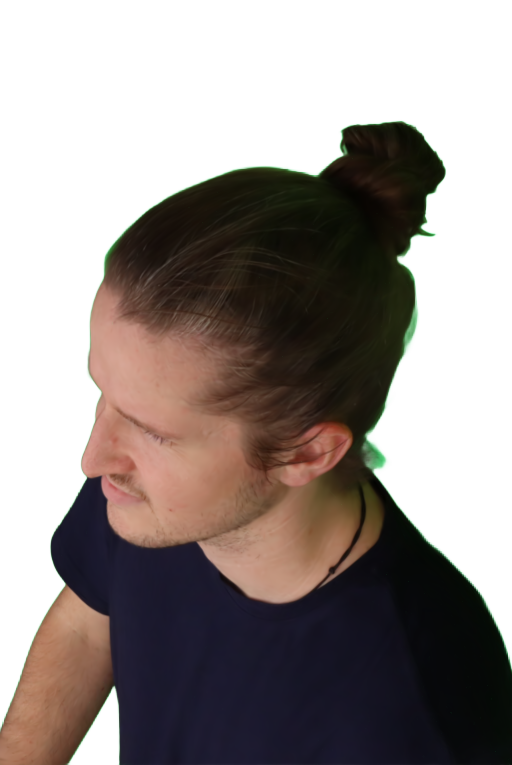
\includegraphics[width=\textwidth]{Figures/results/initials/ephra/22_render.png}
        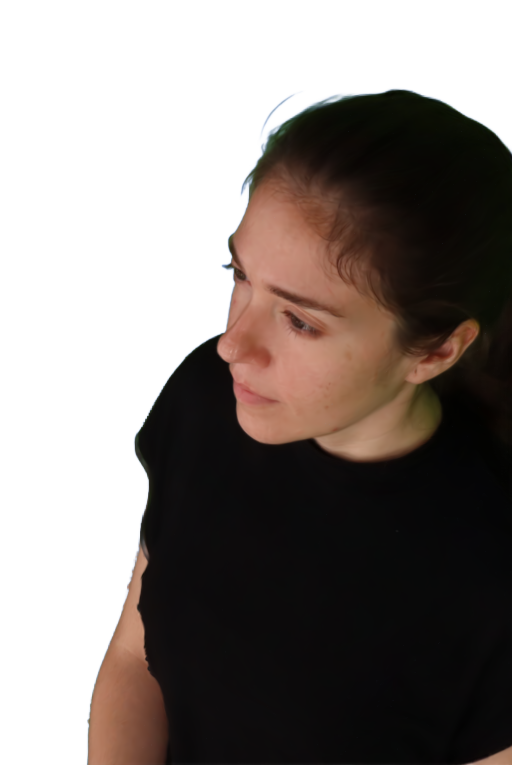
\includegraphics[width=\textwidth]{Figures/results/initials/irene/22_render.png}
        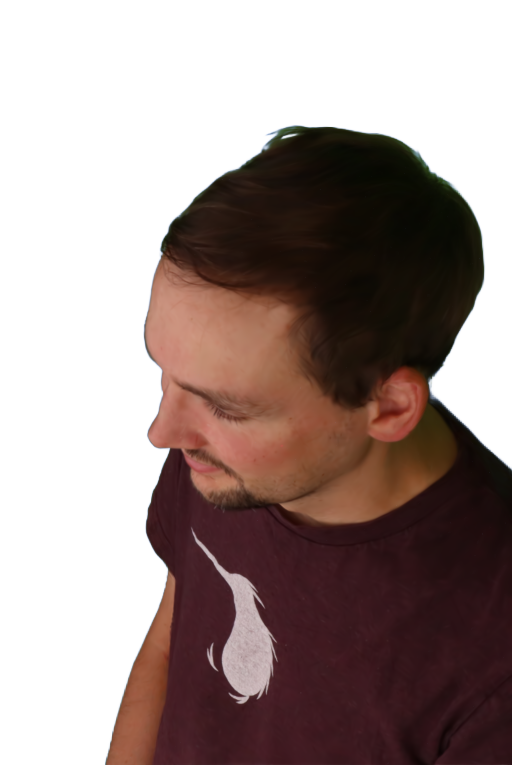
\includegraphics[width=\textwidth]{Figures/results/initials/simon/22_render.png}
	\end{subfigure}
    \caption{From top to bottom: the initial 3D Gaussian Splatting avatars of participant A, B, C, and D. Shown here are views sampled from the training set.}
    \label{fig:igs2gs_init_participants}
\end{figure}

Each of these initial 3D Gaussian Splatting avatars was then stylized using the modified InstructGS2GS method as described in Section \ref{sec:stylization} with high and low textual prompt guidance scale values ($s_P = 7.5$ and $5$, respectively). The initial image guidance scale value $s_I$ determines the influence of the original photographs on the stylization, directly contributing to multi-view stylization (MVS) consistency, as these images are inherently multi-view consistent. Unlike $s_P$, the initial textual guidance scale $s_I$ is solely responsible for the textual prompt's contribution to the stylization. However, both $s_P$ and $s_I$ influence the final stylization result and its MVS consistency. Varying $s_P$ is preferable in this experiment as it tends to produce more diverse and interesting stylization results, highlighting the different tasks various textual prompts contain. Additionally, $s_P$ and $s_I$ may have a trade-off relationship, where a higher $s_P$ may require a lower $s_I$ to maintain MVS consistency, which otherwise might break as mentioned in the previous chapter. The prompts used for stylization and their corresponding tasks are shown in Table \ref{tab:stylization_prompt}.

\begin{table} [H]
	\centering
	\scalebox{0.8}{
		\begin{tabular}{|l|l|l|}
		\hline
		\textbf{ID} &\textbf{Textual Prompt $P$} & \textbf{Type of Stylization Tasks} \\
		\hline
		$P_1$&\textit{"Turn (him/her) into a rabbit"} & Full facial transformation \\
		$P_2$&\textit{"Make (him/her) look like Tolkien Elf"} & Slight facial transformation \\
		$P_3$&\textit{"Turn (him/her) into a stone statue"} & Full recoloring \\
		$P_4$&\textit{"Give (him/her) red hair and blue shirt"} & Partial recoloring \\
		$P_5$&\textit{"Give a cowboy hat"} & Adding visual elements \\
		$P_6$&\textit{"As if a painting in Van Gogh style"} & Well-known art style change \\
		$P_7$&\textit{"Turn into 3D model"} & Generic art style change \\
		$P_8$&\textit{"Have (him/her) smile"} & Facial expression editing \\
		\hline
	\end{tabular}
	}
	\caption{Textual Prompts for Stylization with their respective tasks/expected changes. Usage of the pronoun "him/her" is interchangeable depending on the participant since the InstructPix2Pix model is trained with natural language and is context-aware.}
	\label{tab:stylization_prompt}
\end{table}

\section{Stylization Settings and Results} \label{sec:stylization_settings}

With 8 varied textual prompts $P$ and 2 levels of initial textual guidance scale $s_P$, this experiment produced 16 stylized avatars for each human model, resulting in a total of 64 stylized avatars (SAs). The parameter configurations to create these 64 avatars are summarized in Table \ref{tab:stylized_avatars}. In addition to these two variable parameters, all 64 SAs were produced using the following common hyperparameters:

\begin{itemize}[noitemsep]
	\item Learning rate: 0.05
	\item Culling threshold for transparency $\epsilon_\alpha$: 0.005
	\item Size threshold for pruning the 3D Gaussians $\tau_s$: 0.01
	\item Density threshold for 3D Gaussians $\tau_p$: 0.0008
	\item Initial image guidance scale value $s_I$: 2
	\item Incremental image guidance scale value $\Delta s_I$: 0.2
	\item Incremental textual prompt guidance scale value $\Delta s_P$: 0.55
	\item Negative prompt $P'$ : "low quality, deformed, bad"
	\item Number of iterations: 5000
	\item InstructPix2Pix stylization cycles: 2 (once per 2500 iterations)
\end{itemize}

Rendering samples of the 64 stylized avatars from one of the training views are shown in Figures \ref{fig:all_stylized_results_low} (low $s_P$) and \ref{fig:all_stylized_results_high} (high $s_P$). Refer to the Appendix \ref{AppendixB} for the full sets.

\begin{figure}[ht]
    \centering
	\begin{subfigure}{0.08\linewidth}%rabbit
        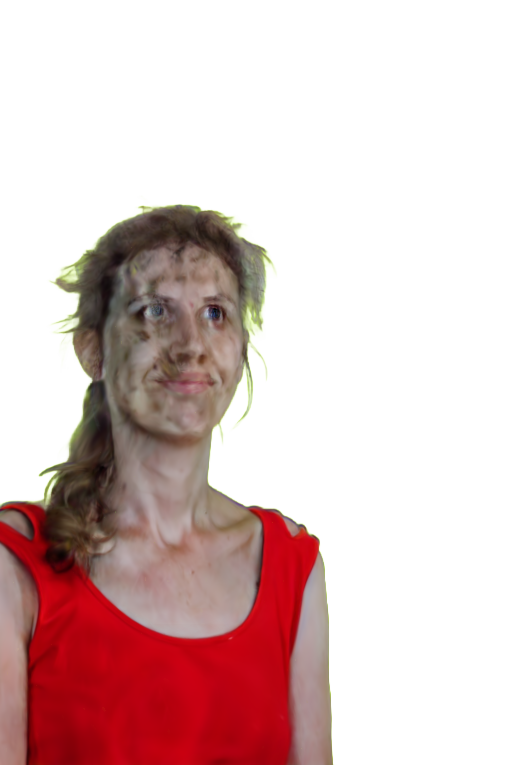
\includegraphics[width=\textwidth]{Figures/results/low/dora_rabbit/11_render.png}
        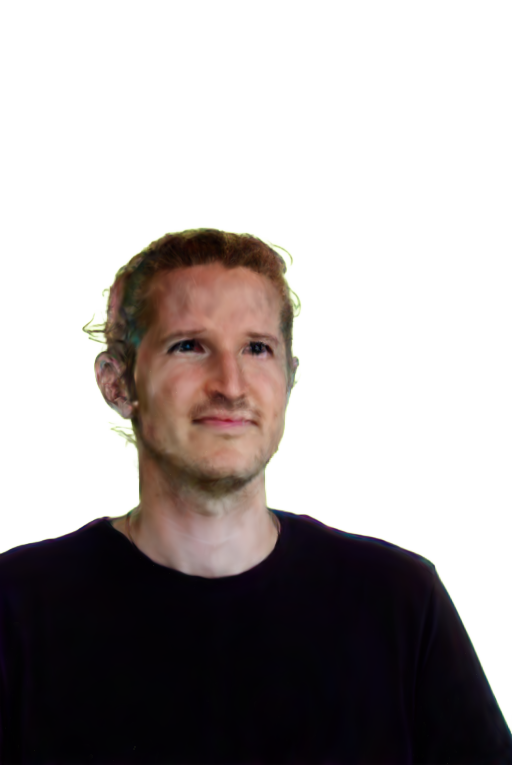
\includegraphics[width=\textwidth]{Figures/results/low/ephra_rabbit/11_render.png}
        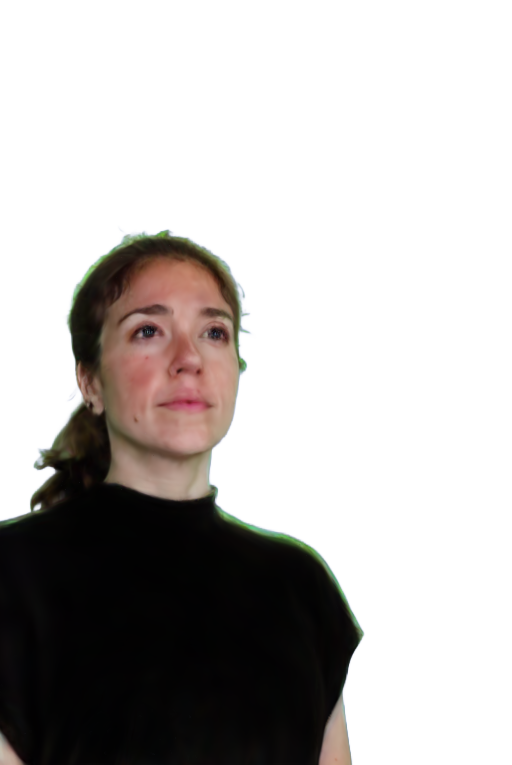
\includegraphics[width=\textwidth]{Figures/results/low/irene_rabbit/11_render.png}
        
\includegraphics[width=\textwidth]{Figures/results/low/simon_rabbit/11_render.png}
	\end{subfigure}
    \begin{subfigure}{0.08\linewidth}%elf
        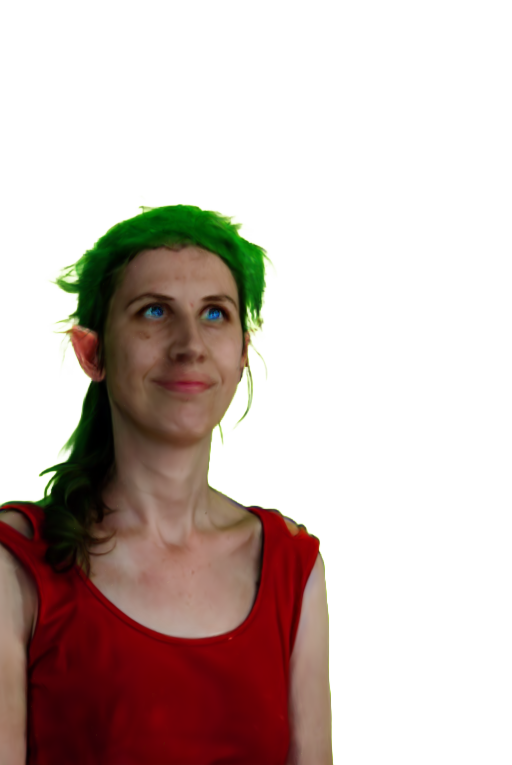
\includegraphics[width=\textwidth]{Figures/results/low/dora_elf/11_render.png}
        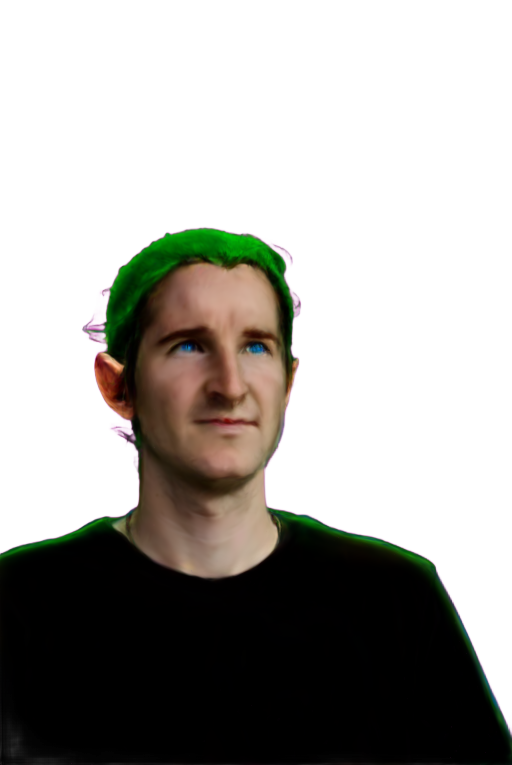
\includegraphics[width=\textwidth]{Figures/results/low/ephra_elf/11_render.png}
        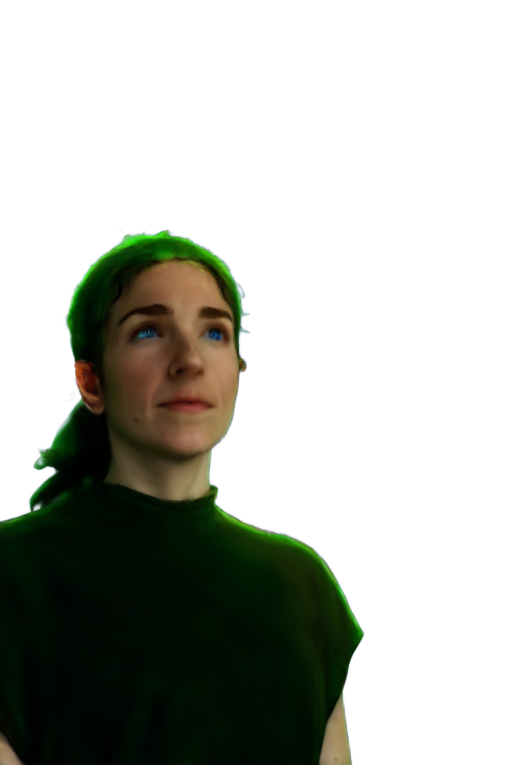
\includegraphics[width=\textwidth]{Figures/results/low/irene_elf/11_render.png}
        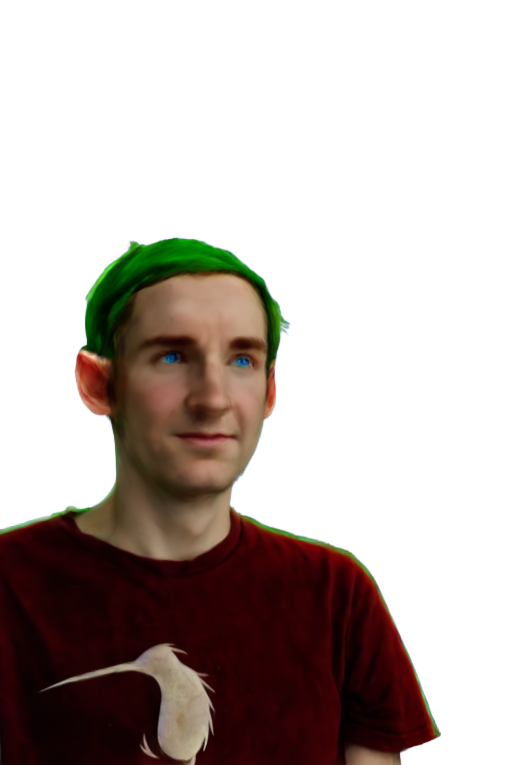
\includegraphics[width=\textwidth]{Figures/results/low/simon_elf/11_render.png}
	\end{subfigure}
    \begin{subfigure}{0.08\linewidth}%stone
        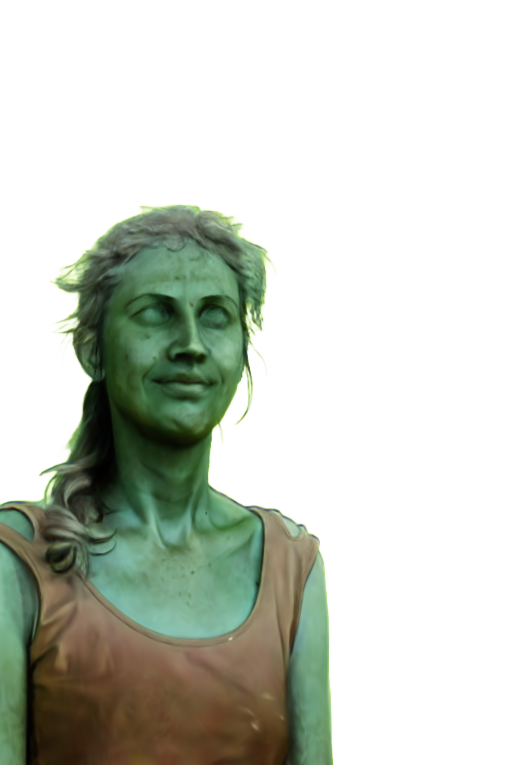
\includegraphics[width=\textwidth]{Figures/results/low/dora_stone/11_render.png}
        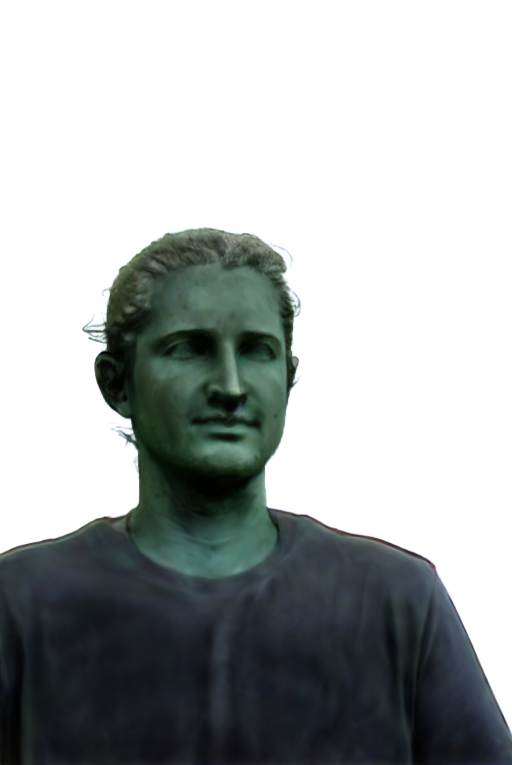
\includegraphics[width=\textwidth]{Figures/results/low/ephra_stone/11_render.png}
        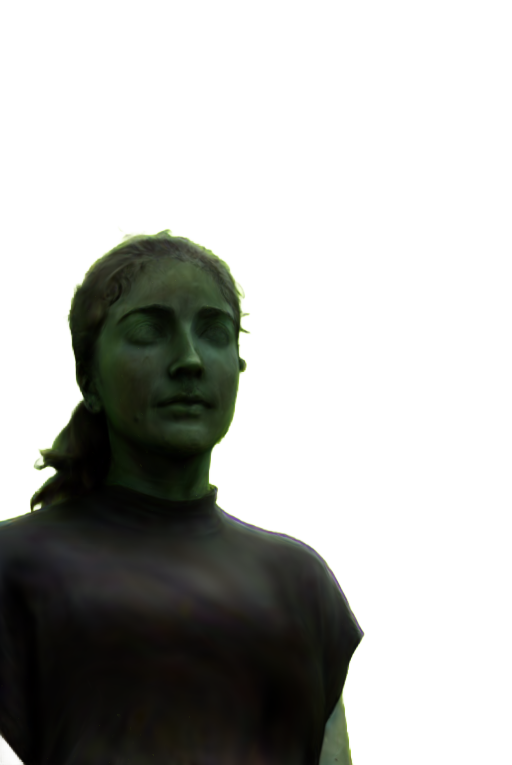
\includegraphics[width=\textwidth]{Figures/results/low/irene_stone/11_render.png}
        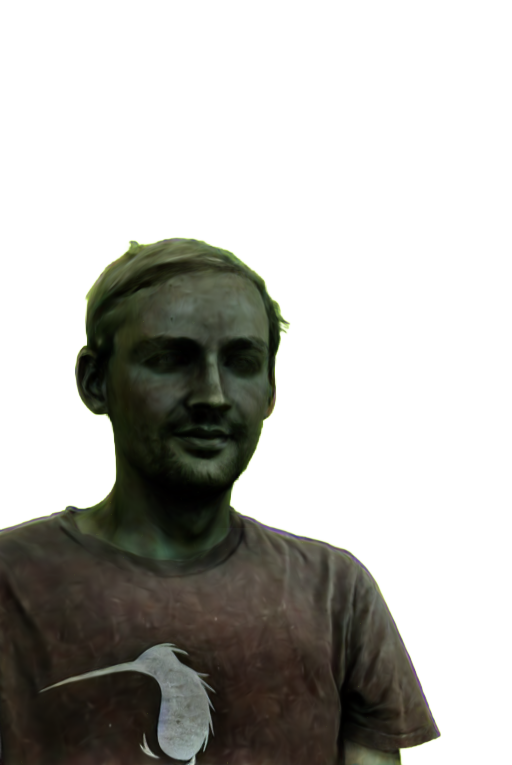
\includegraphics[width=\textwidth]{Figures/results/low/simon_stone/11_render.png}
	\end{subfigure}
    \begin{subfigure}{0.08\linewidth}%red hair
        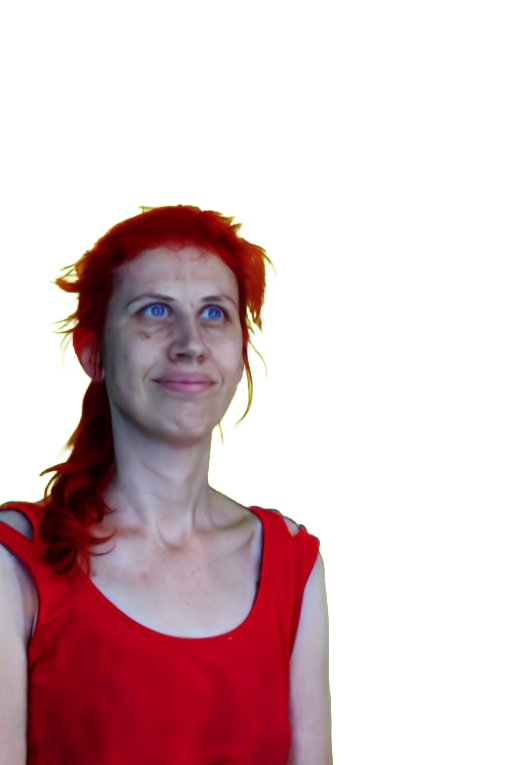
\includegraphics[width=\textwidth]{Figures/results/low/dora_red/11_render.png}
        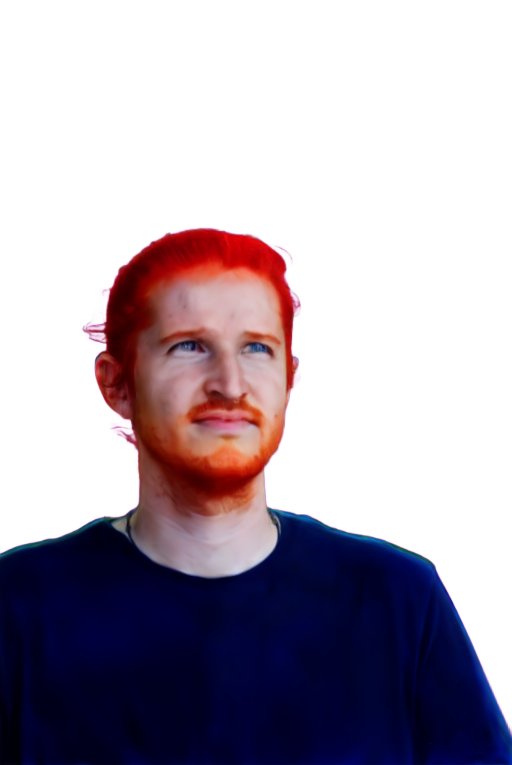
\includegraphics[width=\textwidth]{Figures/results/low/ephra_red/11_render.png}
        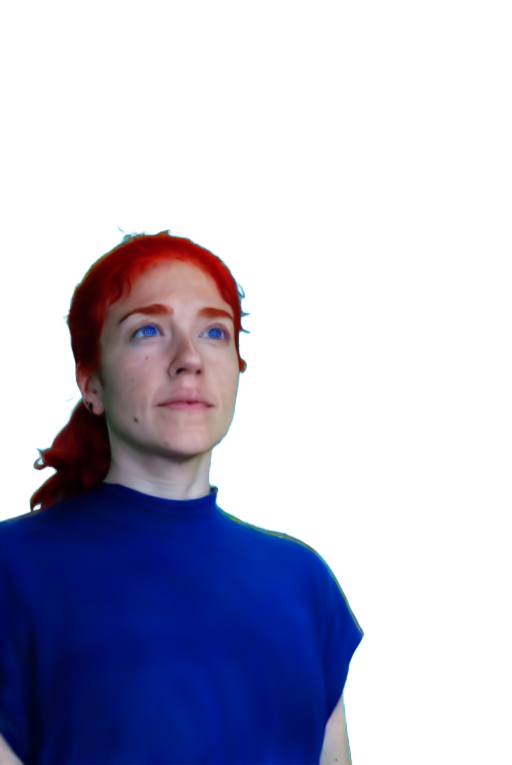
\includegraphics[width=\textwidth]{Figures/results/low/irene_red/11_render.png}
        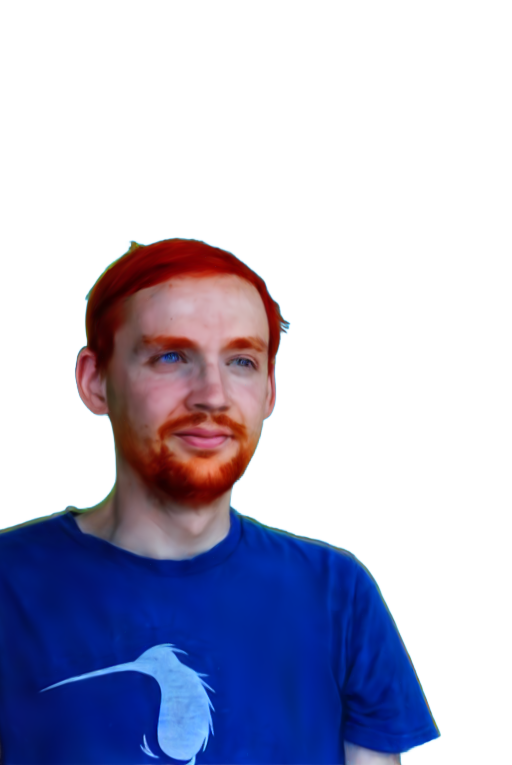
\includegraphics[width=\textwidth]{Figures/results/low/simon_red/11_render.png}
	\end{subfigure}
	\begin{subfigure}{0.08\linewidth}%cowboy
        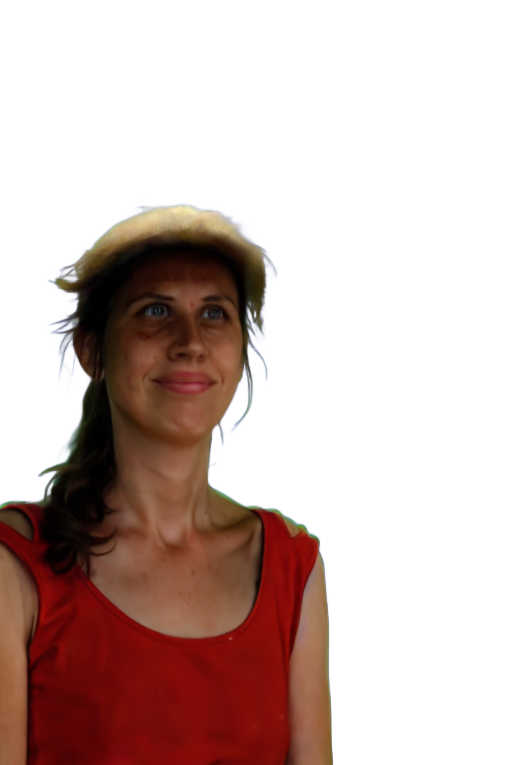
\includegraphics[width=\textwidth]{Figures/results/low/dora_cowboy/11_render.png}
        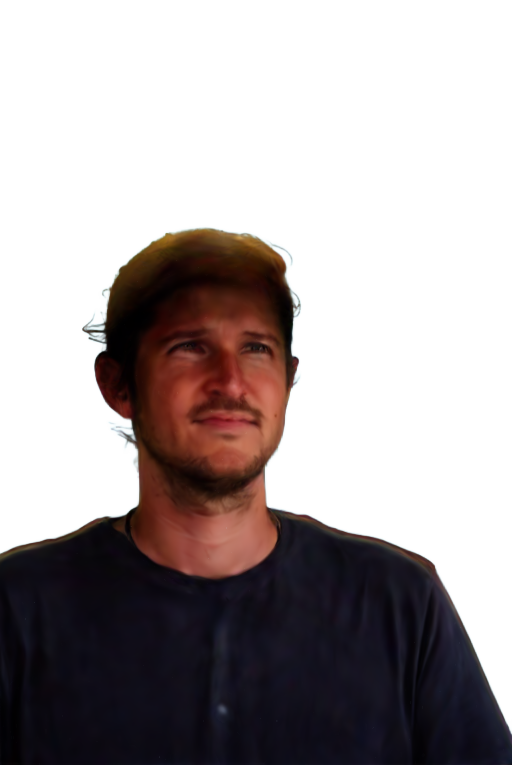
\includegraphics[width=\textwidth]{Figures/results/low/ephra_cowboy/11_render.png}
        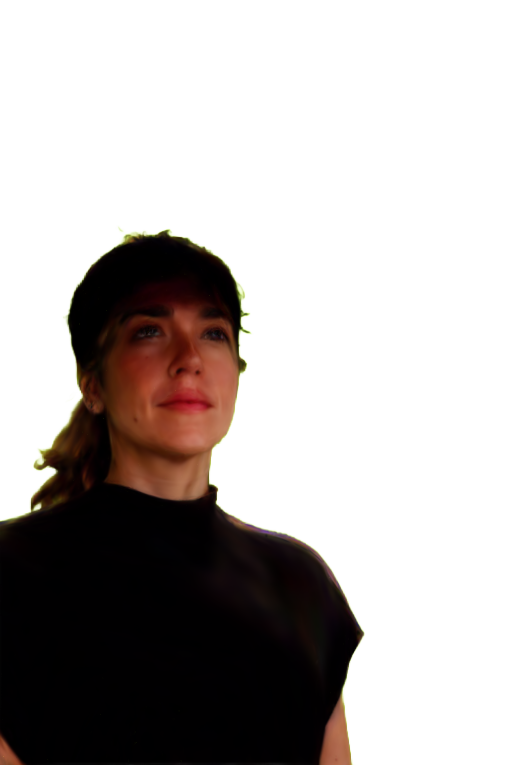
\includegraphics[width=\textwidth]{Figures/results/low/irene_cowboy/11_render.png}
        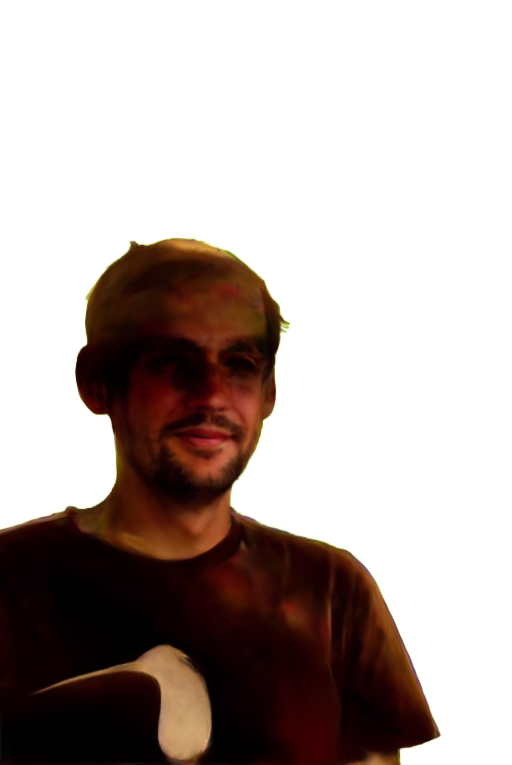
\includegraphics[width=\textwidth]{Figures/results/low/simon_cowboy/11_render.png}
	\end{subfigure}
    \begin{subfigure}{0.08\linewidth}%vangogh
        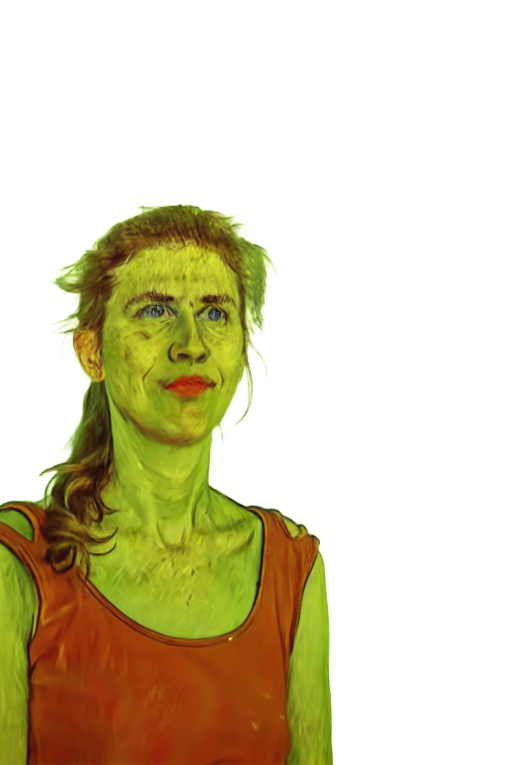
\includegraphics[width=\textwidth]{Figures/results/low/dora_vangogh/11_render.png}
        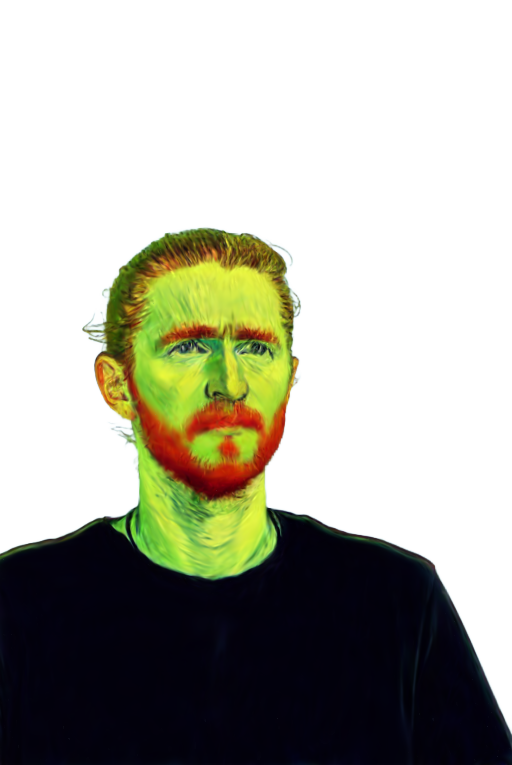
\includegraphics[width=\textwidth]{Figures/results/low/ephra_vangogh/11_render.png}
        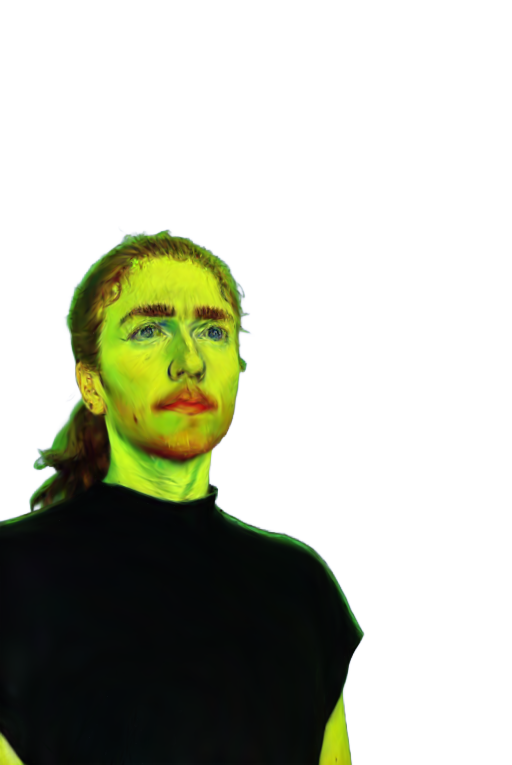
\includegraphics[width=\textwidth]{Figures/results/low/irene_vangogh/11_render.png}
        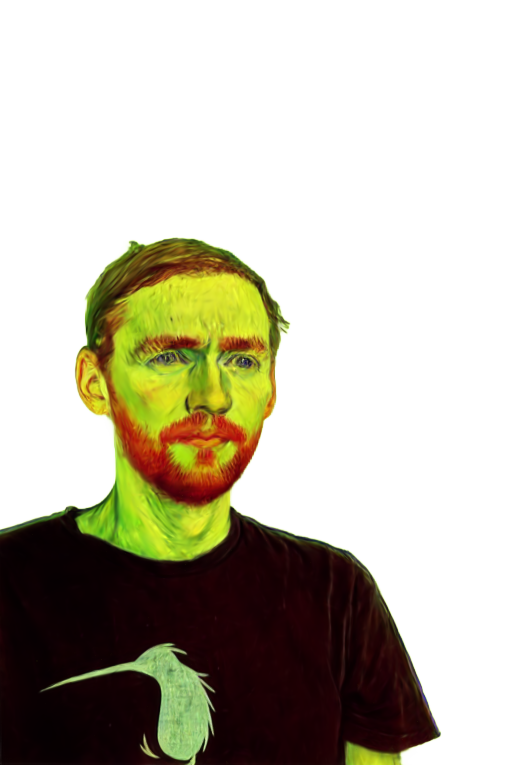
\includegraphics[width=\textwidth]{Figures/results/low/simon_vangogh/11_render.png}
	\end{subfigure}
	\begin{subfigure}{0.08\linewidth}%3dmodel
        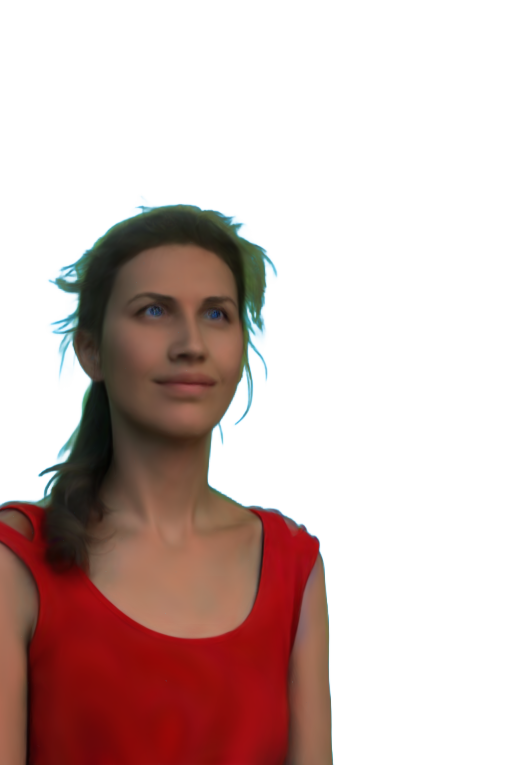
\includegraphics[width=\textwidth]{Figures/results/low/dora_3d/11_render.png}
        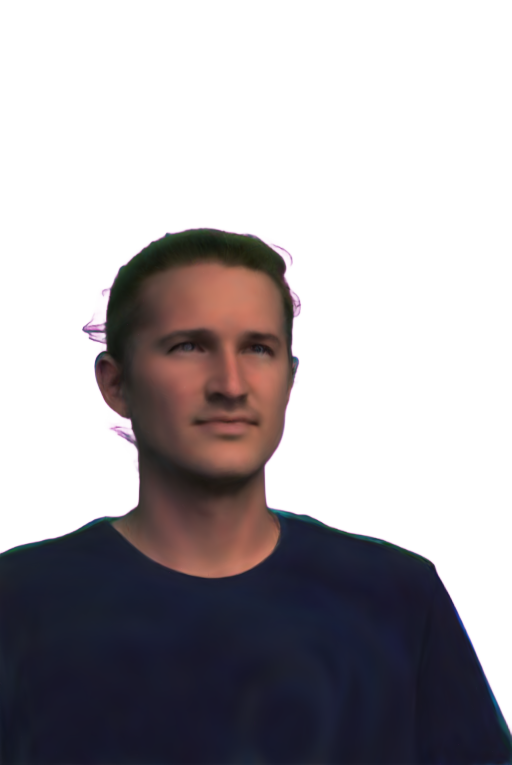
\includegraphics[width=\textwidth]{Figures/results/low/ephra_3d/11_render.png}
        \includegraphics[width=\textwidth]{Figures/results/low/irene_3d/11_render.png}
        \includegraphics[width=\textwidth]{Figures/results/low/simon_3d/11_render.png}
	\end{subfigure}
    \begin{subfigure}{0.08\linewidth}%smile
        \includegraphics[width=\textwidth]{Figures/results/low/dora_smile/11_render.png}
        \includegraphics[width=\textwidth]{Figures/results/low/ephra_smile/11_render.png}
        \includegraphics[width=\textwidth]{Figures/results/low/irene_smile/11_render.png}
        \includegraphics[width=\textwidth]{Figures/results/low/simon_smile/11_render.png}
	\end{subfigure}
    \caption{From top left to bottom right: the stylized avatars (SA) of configuration 1 to 32.}
    \label{fig:all_stylized_results_low}
\end{figure}

\begin{figure}[ht]
    \centering
	\begin{subfigure}{0.08\linewidth}%rabbit
        \includegraphics[width=\textwidth]{Figures/results/high/dora_rabbit/11_render.png}
        \includegraphics[width=\textwidth]{Figures/results/high/ephra_rabbit/11_render.png}
        \includegraphics[width=\textwidth]{Figures/results/high/irene_rabbit/11_render.png}
        \includegraphics[width=\textwidth]{Figures/results/high/simon_rabbit/11_render.png}
	\end{subfigure}
    \begin{subfigure}{0.08\linewidth}%elf
        \includegraphics[width=\textwidth]{Figures/results/high/ephra_elf/11_render.png}
        \includegraphics[width=\textwidth]{Figures/results/high/irene_elf/11_render.png}
        \includegraphics[width=\textwidth]{Figures/results/high/dora_elf/11_render.png}
        \includegraphics[width=\textwidth]{Figures/results/high/simon_elf/11_render.png}
	\end{subfigure}
    \begin{subfigure}{0.08\linewidth}%stone
        \includegraphics[width=\textwidth]{Figures/results/high/dora_stone/11_render.png}
        \includegraphics[width=\textwidth]{Figures/results/high/ephra_stone/11_render.png}
        \includegraphics[width=\textwidth]{Figures/results/high/irene_stone/11_render.png}
        \includegraphics[width=\textwidth]{Figures/results/high/simon_stone/11_render.png}
	\end{subfigure}
    \begin{subfigure}{0.08\linewidth}%red hair
        \includegraphics[width=\textwidth]{Figures/results/high/dora_red/11_render.png}
        \includegraphics[width=\textwidth]{Figures/results/high/ephra_red/11_render.png}
        \includegraphics[width=\textwidth]{Figures/results/high/irene_red/11_render.png}
        \includegraphics[width=\textwidth]{Figures/results/high/simon_red/11_render.png}
	\end{subfigure}
	\begin{subfigure}{0.08\linewidth}%cowboy
        \includegraphics[width=\textwidth]{Figures/results/high/dora_cowboy/11_render.png}
        \includegraphics[width=\textwidth]{Figures/results/high/ephra_cowboy/11_render.png}
        \includegraphics[width=\textwidth]{Figures/results/high/irene_cowboy/11_render.png}
        \includegraphics[width=\textwidth]{Figures/results/high/simon_cowboy/11_render.png}
	\end{subfigure}
    \begin{subfigure}{0.08\linewidth}%vangogh
        \includegraphics[width=\textwidth]{Figures/results/high/dora_vangogh/11_render.png}
        \includegraphics[width=\textwidth]{Figures/results/high/ephra_vangogh/11_render.png}
        \includegraphics[width=\textwidth]{Figures/results/high/irene_vangogh/11_render.png}
        \includegraphics[width=\textwidth]{Figures/results/high/simon_vangogh/11_render.png}
	\end{subfigure}
	\begin{subfigure}{0.08\linewidth}%3dmodel
        \includegraphics[width=\textwidth]{Figures/results/high/dora_3d/11_render.png}
        \includegraphics[width=\textwidth]{Figures/results/high/ephra_3d/11_render.png}
        \includegraphics[width=\textwidth]{Figures/results/high/irene_3d/11_render.png}
        \includegraphics[width=\textwidth]{Figures/results/high/simon_3d/11_render.png}
	\end{subfigure}
    \begin{subfigure}{0.08\linewidth}%smile
        \includegraphics[width=\textwidth]{Figures/results/high/dora_smile/11_render.png}
        \includegraphics[width=\textwidth]{Figures/results/high/ephra_smile/11_render.png}
        \includegraphics[width=\textwidth]{Figures/results/high/irene_smile/11_render.png}
        \includegraphics[width=\textwidth]{Figures/results/high/simon_smile/11_render.png}
	\end{subfigure}
	\caption{From top left to bottom right: the stylized avatars (SA) of configuration 33 to 64.}
    \label{fig:all_stylized_results_high}
\end{figure}

\section{Qualitative Evaluation}
These 64 stylized avatars (SAs) were evaluated qualitatively (e.g., how noticeable are deformation/artifacts/shape changes/color inconsistencies across views). Each SA was assigned a score from 1 to 3, categorized based on its MVS consistency level: poorly consistent (1), moderately consistent (2), and highly consistent (3). An additional category, "failure-case" (score 0), was included for SAs that were either improperly stylized or failed to achieve the stylization task outlined in Table \ref{tab:stylization_prompt}. The results are shown in Table \ref{tab:stylized_avatars}.

\begin{table}[ht]
	\centering
	\scalebox{0.55}{

	\begin{tabular}{|c|c|c|c|c|}
	\hline
	\textbf{SA} & \textbf{M} & \textbf{P} & \textbf{$S_P$} & \textbf{Quality} \\
	\hline
	1                & A            & P1              & low & 1\\
	2                & A            & P2              & low & 2\\
	3                & A            & P3              & low & 3\\
	4                & A            & P4              & low & 2\\
	5                & A            & P5              & low & 1\\
	6                & A            & P6              & low & 2\\
	7                & A            & P7              & low & 3\\
	8                & A            & P8              & low & 1\\
	9                & B            & P1              & low & 1\\
	10               & B            & P2              & low & 3\\
	11               & B            & P3              & low & 3\\
	12               & B            & P4              & low & 3\\
	13               & B            & P5              & low & 1\\
	14               & B            & P6              & low & 2\\
	15               & B            & P7              & low & 3\\
	16               & B            & P8              & low & 1\\
	\hline
	\end{tabular}
	}
	\quad
	\scalebox{0.55}{
	\begin{tabular}{|c|c|c|c|c|}
	\hline
	\textbf{SA} & \textbf{M} & \textbf{P} & \textbf{$S_P$} & \textbf{Quality} \\
	\hline
	17               & C            & P1              & low & 0\\
	18               & C            & P2              & low & 3\\
	19               & C            & P3              & low & 3\\
	20               & C            & P4              & low & 3\\
	21               & C            & P5              & low & 1\\
	22               & C            & P6              & low & 3\\
	23               & C            & P7              & low & 3\\
	24               & C            & P8              & low & 1\\
	25               & D            & P1              & low & 0\\
	26               & D            & P2              & low & 1\\
	27               & D            & P3              & low & 3\\
	28               & D            & P4              & low & 3\\
	29               & D            & P5              & low & 1\\
	30               & D            & P6              & low & 3\\
	31               & D            & P7              & low & 3\\
	32               & D            & P8              & low & 1\\
	\hline
	\end{tabular}
	}
	\quad
	\scalebox{0.55}{
	\begin{tabular}{|c|c|c|c|c|}
	\hline
	\textbf{SA} & \textbf{M} & \textbf{P} & \textbf{$S_P$} & \textbf{Quality} \\
	\hline
	33               & A            & P1              & high& 1\\
	34               & A            & P2              & high& 1\\
	35               & A            & P3              & high& 3\\
	36               & A            & P4              & high& 2\\
	37               & A            & P5              & high& 1\\
	38               & A            & P6              & high& 2\\
	39               & A            & P7              & high& 2\\
	40               & A            & P8              & high& 1\\
	41               & B            & P1              & high& 1\\
	42               & B            & P2              & high& 2\\
	43               & B            & P3              & high& 3\\
	44               & B            & P4              & high& 3\\
	45               & B            & P5              & high& 1\\
	46               & B            & P6              & high& 2\\
	47               & B            & P7              & high& 1\\
	48               & B            & P8              & high& 1\\
	\hline
	\end{tabular}
	}
	\quad
	\scalebox{0.55}{
	\begin{tabular}{|c|c|c|c|c|}
	\hline
	\textbf{SA} & \textbf{M} & \textbf{P} & \textbf{$S_P$} & \textbf{Quality} \\
	\hline
	49               & C            & P1              & high& 1\\
	50               & C            & P2              & high& 2\\
	51               & C            & P3              & high& 2\\
	52               & C            & P4              & high& 2\\
	53               & C            & P5              & high& 1\\
	54               & C            & P6              & high& 2\\
	55               & C            & P7              & high& 2\\
	56               & C            & P8              & high& 1\\
	57               & D            & P1              & high& 0\\
	58               & D            & P2              & high& 2\\
	59               & D            & P3              & high& 3\\
	60               & D            & P4              & high& 3\\
	61               & D            & P5              & high& 1\\
	62               & D            & P6              & high& 2\\
	63               & D            & P7              & high& 2\\
	64               & D            & P8              & high& 1\\
	\hline
	\end{tabular}
	}
	\caption{All configurations of the stylized avatars used in this thesis, along with their qualitative stylization consistency. SA stands for Stylized Avatar. Human models (M) are denoted as A, B, C, and D. $P$ stands for the textual prompt used for stylization. $s_P$ stands for the textual prompt guidance scale value (5 for low and 7.5 for high). Quality is the qualitative evaluation of the stylized avatar with a range from 1 (poorly consistent) to 3 (highly consistent), with 0 as failure-case.}
	\label{tab:stylized_avatars}
\end{table}

\begin{figure}[ht]
	\centering
	\includegraphics[width=0.6\textwidth]{Figures/results/qualitative distribution.png}
	\caption{Distribution of MVS consistency of the stylized avatars based on qualitative evaluation.}
	\label{fig:qualitative_distribution}
\end{figure}

Figure \ref{fig:qualitative_distribution} shows the qualitative distribution of the stylized avatars based on their MVS consistency levels with respect to the initial textual guidance scale $s_P$. This distribution indicates that stylized avatars with better MVS consistency are more likely produced with configurations using a low initial textual guidance scale $s_P$. This is expected, as discussed in the previous chapter. The initial textual guidance scale $s_P$ adversely affects MVS consistency, with the number of SAs showing poor or moderate MVS consistency increasing and those with high MVS consistency decreasing as $s_P$ rises. This trend is also evident in Figure \ref{fig:MVS_consistency_change}, with a noticeable downward trend in MVS consistency from right to left (low to high $s_P$).

Interestingly, the number of poorly consistent SAs is comparably high in configurations with both high and low $s_P$. This high number of poorly consistent results is due to the limitations of the InstructPix2Pix model, which cannot sufficiently stylize some prompts. Upon further inspection, prompts $P_5$ and $P_8$ consistently produce MVS inconsistent results. The most problematic, however, is prompt $P_1$, which often results in failure-case SAs or poor MVS. Although a decrease in failure cases is observed between low and high $s_P$, this reduction is somewhat misleading, as the corresponding SAs exhibit poor MVS consistency (see SAs 17 and 49 in Table \ref{tab:stylized_avatars} and the upward trend in Figure \ref{fig:MVS_consistency_change} for Model C). As shown in Figure \ref{fig:MVS_consistency_change}, the MVS consistency produced by these three prompts nearly always occupies the bottom portion of each chart, regardless of the $s_P$ value used. The stylizations with the remaining text prompts ($P_2, P_3, P_4, P_6, P_7$) generally produce SAs with better MVS consistency under low $s_P$ than high $s_P$, as expected. The raw data for all values presented in the next section can be found in Appendix \ref{AppendixA}.

\begin{figure}[h]
	\centering
	\begin{subfigure}{0.24\linewidth}
		\includegraphics[width=\textwidth]{Figures/results/qualitative_A.png}
		\caption{Model A}
	\end{subfigure}
	\begin{subfigure}{0.24\linewidth}
		\includegraphics[width=\textwidth]{Figures/results/qualitative_B.png}
		\caption{Model B}
	\end{subfigure}
	\begin{subfigure}{0.24\linewidth}
		\includegraphics[width=\textwidth]{Figures/results/qualitative_C.png}
		\caption{Model C}
	\end{subfigure}
	\begin{subfigure}{0.24\linewidth}
		\includegraphics[width=\textwidth]{Figures/results/qualitative_D.png}
		\caption{Model D}
	\end{subfigure}
	\caption{Change in qualitative MVS consistency for each human model based on the textual prompt guidance scale $s_P$ for each prompt $P$. The two parallel vertical axes represent the qualitative MVS consistency level (the higher, the better) for both levels of textual prompt guidance scale $s_P$. The horizontal lines represent the change for each prompt between high and low $s_P$.}
	\label{fig:MVS_consistency_change}

\end{figure}

This is likely due to prompt $P_1$ forcing a full facial transformation, expecting significant changes in content (human to animal). This task is challenging for the InstructPix2Pix model, as it was trained with a limited dataset and cannot generalize well to this specific type of stylization. Figure \ref{fig:failed_rabbit} shows an example of failed/poor stylization.

\begin{figure}[ht]
	\centering
	\begin{subfigure}{0.2\linewidth}
		\includegraphics[width=\textwidth]{Figures/failed/rabbit/3_render-removebg-preview.png}
	\end{subfigure}
	\begin{subfigure}{0.2\linewidth}
		\includegraphics[width=\textwidth]{Figures/failed/rabbit/5_render-removebg-preview.png}
	\end{subfigure}
	\begin{subfigure}{0.2\linewidth}
		\includegraphics[width=\textwidth]{Figures/failed/rabbit/32_render-removebg-preview.png}
	\end{subfigure}
	\begin{subfigure}{0.2\linewidth}
		\includegraphics[width=\textwidth]{Figures/failed/rabbit/34_render-removebg-preview.png}
	\end{subfigure}
	\caption{Rendering from 4 neighboring views of the failed stylized avatar (SA 9) with prompt $P_1$ for human model B. There is obvious stylization inconsistency across the views, but color changes are not significant enough for $\mathsf{RMSE}_{t}$ and $\Delta E_{00,t}$.}
	\label{fig:failed_rabbit}
\end{figure}

\begin{figure}[ht]
	\centering
	\begin{subfigure}{0.2\linewidth}
		\includegraphics[width=\textwidth]{Figures/failed/cowboy/15_render-removebg-preview.png}
	\end{subfigure}
	\begin{subfigure}{0.2\linewidth}
		\includegraphics[width=\textwidth]{Figures/failed/cowboy/16_render-removebg-preview.png}
	\end{subfigure}
	\begin{subfigure}{0.2\linewidth}
		\includegraphics[width=\textwidth]{Figures/failed/cowboy/17_render-removebg-preview.png}
	\end{subfigure}
	\begin{subfigure}{0.2\linewidth}
		\includegraphics[width=\textwidth]{Figures/failed/cowboy/18_render-removebg-preview.png}
	\end{subfigure}
	\caption{Rendering from 4 neighboring views of the failed stylized avatar (SA 13) with prompt $P_5$ for human model B. There is stylization inconsistency across the views and significant color changes from the neighboring views.}
	\label{fig:failed_cowboy}
\end{figure}

\begin{figure}[ht]
	\centering
	\begin{subfigure}{0.2\linewidth}
		\includegraphics[width=\textwidth]{Figures/failed/smile/2_render-removebg-preview.png}
	\end{subfigure}
	\begin{subfigure}{0.2\linewidth}
		\includegraphics[width=\textwidth]{Figures/failed/smile/3_render-removebg-preview.png}
	\end{subfigure}
	\begin{subfigure}{0.2\linewidth}
		\includegraphics[width=\textwidth]{Figures/failed/smile/5_render-removebg-preview.png}
	\end{subfigure}
	\begin{subfigure}{0.2\linewidth}
		\includegraphics[width=\textwidth]{Figures/failed/smile/6_render-removebg-preview.png}
	\end{subfigure}
	\caption{The renderings from 4 neighboring views of the failed stylized avatar (SA 48) with prompt $P_8$ for human model B. Inconsistency in facial expression is easily perceivable, but there are not many color changes detected by $\mathsf{RMSE}_{t}$ and $\Delta E_{00,t}$.}
	\label{fig:failed_smile}
\end{figure}

The next section discusses the quantitative evaluation of the stylized avatars and how the MVS consistency measured by this method correlates with the qualitative evaluation.

\section{Quantitative Evaluation}
The quantitative evaluation of the SAs employs the camera-specific metrics described in Section \ref{sec:metric}, namely $\mathsf{LPIPS}_{t}$, $\mathsf{RMSE}_{t}$, and $\Delta E_{00,t}$. This section analyzes the distribution of these metric values across views to assess the MVS consistency of the stylized avatars quantitatively and determine alignment with qualitative observations.

\subsection{Low and high $s_P$ in relation to MVS consistency metrics}

\begin{figure}[ht]
	\centering
	\begin{subfigure}{0.49\textwidth}
		\includegraphics[width=\linewidth]{Figures/results/good/lpips_dora.png}
		\caption{From top to bottom: SA 2, 34, 3, 35, 4, 36, 6, 38, 7, and 39}
	\end{subfigure}
	\begin{subfigure}{0.49\textwidth}
		\includegraphics[width=\linewidth]{Figures/results/good/lpips_ephra.png}
		\caption{From top to bottom: SA 10, 42, 11, 43, 12, 44, 14, 46, 15, and 47}
	\end{subfigure}
	\begin{subfigure}{0.49\textwidth}
		\includegraphics[width=\linewidth]{Figures/results/good/lpips_irene.png}
		\caption{From top to bottom: SA 18, 50, 19, 51, 20, 52, 22, 54, 23, and 55}
	\end{subfigure}
	\begin{subfigure}{0.49\textwidth}
		\includegraphics[width=\linewidth]{Figures/results/good/lpips_simon.png}
		\caption{From top to bottom: SA 26, 58, 27, 59, 28, 60, 30, 62, 31, and 63}
	\end{subfigure}
	\caption{Distribution of the $\mathsf{LPIPS}_{t}$ values across the view for each human model, grouped by the level of textual prompt guidance scale $s_P$ for $P_3$, $P_4$, $P_6$, and $P_7$. Empty circles indicate the outliers.}
	\label{fig:quantitative_distribution_lpips_good}
\end{figure}

\begin{figure}[ht]
	\centering
	\begin{subfigure}{0.49\textwidth}
		\includegraphics[width=\linewidth]{Figures/results/good/rmse_dora.png}
		\caption{From top to bottom: SA 2, 34, 3, 35, 4, 36, 6, 38, 7, and 39}
		\label{fig:rmse_dora}
	\end{subfigure}
	\begin{subfigure}{0.49\textwidth}
		\includegraphics[width=\linewidth]{Figures/results/good/rmse_ephra.png}
		\caption{From top to bottom: SA 10, 42, 11, 43, 12, 44, 14, 46, 15, and 47}
		\label{fig:rmse_ephra}
	\end{subfigure}
	\begin{subfigure}{0.49\textwidth}
		\includegraphics[width=\linewidth]{Figures/results/good/rmse_irene.png}
		\caption{From top to bottom: SA 18, 50, 19, 51, 20, 52, 22, 54, 23, and 55}
		\label{fig:rmse_irene}
	\end{subfigure}
	\begin{subfigure}{0.49\textwidth}
		\includegraphics[width=\linewidth]{Figures/results/good/rmse_simon.png}
		\caption{From top to bottom: SA 26, 58, 27, 59, 28, 60, 30, 62, 31, and 63}
		\label{fig:rmse_simon}
	\end{subfigure}
	\caption{Distribution of the $\mathsf{RMSE}_{t}$ values across the view for each human model, grouped by the level of textual prompt guidance scale $s_P$ for $P_3$, $P_4$, $P_6$, and $P_7$. Empty circles indicate the outliers.}
	\label{fig:quantitative_distribution_rmse_good}
\end{figure}

\begin{figure}[ht]
	\centering
	\begin{subfigure}{0.49\textwidth}
		\includegraphics[width=\linewidth]{Figures/results/good/ciede2000_dora.png}
		\caption{Top to bottom: SA 2, 34, 3, 35, 4, 36, 6, 38, 7, and 39}
		\label{fig:ciede2000_dora}
	\end{subfigure}
	\begin{subfigure}{0.49\textwidth}
		\includegraphics[width=\linewidth]{Figures/results/good/ciede2000_ephra.png}
		\caption{Top to bottom: SA 10, 42, 11, 43, 12, 44, 14, 46, 15, and 47}
		\label{fig:ciede2000_ephra}
	\end{subfigure}
	\begin{subfigure}{0.49\textwidth}
		\includegraphics[width=\linewidth]{Figures/results/good/ciede2000_irene.png}
		\caption{Top to bottom: SA 18, 50, 19, 51, 20, 52, 22, 54, 23, and 55}
		\label{fig:ciede2000_irene}
	\end{subfigure}
	\begin{subfigure}{0.49\textwidth}
		\includegraphics[width=\linewidth]{Figures/results/good/ciede2000_simon.png}
		\caption{Top to bottom: SA 26, 58, 27, 59, 28, 60, 30, 62, 31, and 63}
		\label{fig:ciede2000_simon}
	\end{subfigure}
	\caption{Distribution of the $\Delta E_{00}$ values across the view for each human model, grouped by the level of textual prompt guidance scale $s_P$ for $P_3$, $P_4$, $P_6$, and $P_7$. Empty circles indicate the outliers.}
	\label{fig:quantitative_distribution_ciede2000_good}
\end{figure}

Observing that certain textual prompts (P1, P5, and P8, as shown in Figures \ref{fig:failed_rabbit}, \ref{fig:failed_cowboy}, and \ref{fig:failed_smile}, respectively) consistently produce qualitatively poor MVS consistency, initial quantitative comparisons focused on SAs created with the remaining prompts ($P_3$, $P_2$, $P_4$, $P_6$, and $P_7$) under low and high $s_P$ settings. This amounts to 40 experimental results for each metric.

For each model, associated SAs are measured using the three metrics, and values from each camera are collated. The arithmetic mean, second, and third quartiles are calculated. In addition to the SAs, the initial 3D Gaussian Splatting avatars are measured as a reference point to showcase how these metrics perform on results with "perfect" MVS consistency. The distribution of $\mathsf{LPIPS}_{t}$, $\mathsf{RMSE}_{t}$, and $\Delta E_{00,t}$ are shown in Figures \ref{fig:quantitative_distribution_lpips_good}, \ref{fig:quantitative_distribution_rmse_good}, and \ref{fig:quantitative_distribution_ciede2000_good} as box plots, respectively. Lower values of these metrics indicate higher MVS consistency of the SAs. To better understand the values given by these metrics, standard deviations are also computed and shown alongside the averages for each associated SA in Figures \ref{fig:sd_quantitative_distribution_lpips_good}, \ref{fig:sd_quantitative_distribution_rmse_good}, and \ref{fig:sd_quantitative_distribution_ciede2000_good}.

\begin{figure}[ht]
	\centering
	\begin{subfigure}{0.49\textwidth}
		\includegraphics[width=\linewidth]{Figures/results/good/sd_lpips_dora.png}
		\caption{From top to bottom: SA 2, 34, 3, 35, 4, 36, 6, 38, 7, and 39}
	\end{subfigure}
	\begin{subfigure}{0.49\textwidth}
		\includegraphics[width=\linewidth]{Figures/results/good/sd_lpips_ephra.png}
		\caption{From top to bottom: SA 10, 42, 11, 43, 12, 44, 14, 46, 15, and 47}
	\end{subfigure}
	\begin{subfigure}{0.49\textwidth}
		\includegraphics[width=\linewidth]{Figures/results/good/sd_lpips_irene.png}
		\caption{From top to bottom: SA 18, 50, 19, 51, 20, 52, 22, 54, 23, and 55}
	\end{subfigure}
	\begin{subfigure}{0.49\textwidth}
		\includegraphics[width=\linewidth]{Figures/results/good/sd_lpips_simon.png}
		\caption{From top to bottom: SA 26, 58, 27, 59, 28, 60, 30, 62, 31, and 63}
	\end{subfigure}
	\caption{Standard deviation of the $\mathsf{LPIPS}_{t}$ and the $\mathsf{LPIPS}(\varGamma)$ values across the view for each human model, grouped by the level of textual prompt guidance scale $s_P$ for $P_3$, $P_4$, $P_6$ and $P_7$.}
	\label{fig:sd_quantitative_distribution_lpips_good}
\end{figure}

\begin{figure}[ht]
	\centering
	\begin{subfigure}{0.49\textwidth}
		\includegraphics[width=\linewidth]{Figures/results/good/sd_rmse_dora.png}
		\caption{From top to bottom: SA 2, 34, 3, 35, 4, 36, 6, 38, 7, and 39}
	\end{subfigure}
	\begin{subfigure}{0.49\textwidth}
		\includegraphics[width=\linewidth]{Figures/results/good/sd_rmse_ephra.png}
		\caption{From top to bottom: SA 10, 42, 11, 43, 12, 44, 14, 46, 15, and 47}
	\end{subfigure}
	\begin{subfigure}{0.49\textwidth}
		\includegraphics[width=\linewidth]{Figures/results/good/sd_rmse_irene.png}
		\caption{From top to bottom: SA 18, 50, 19, 51, 20, 52, 22, 54, 23, and 55}
	\end{subfigure}
	\begin{subfigure}{0.49\textwidth}
		\includegraphics[width=\linewidth]{Figures/results/good/sd_rmse_simon.png}
		\caption{From top to bottom: SA 26, 58, 27, 59, 28, 60, 30, 62, 31, and 63}
	\end{subfigure}
	\caption{Standard deviation of the $\mathsf{RMSE}_{t}$ and the $\mathsf{RMSE}(\varGamma)$ values across the view for each human model, grouped by the level of textual prompt guidance scale $s_P$ for $P_3$, $P_4$, $P_6$ and $P_7$.}
	\label{fig:sd_quantitative_distribution_rmse_good}
\end{figure}

\begin{figure}[ht]
	\centering
	\begin{subfigure}{0.49\textwidth}
		\includegraphics[width=\linewidth]{Figures/results/good/sd_ciede2000_dora.png}
		\caption{From top to bottom: SA 2, 34, 3, 35, 4, 36, 6, 38, 7, and 39}
	\end{subfigure}
	\begin{subfigure}{0.49\textwidth}
		\includegraphics[width=\linewidth]{Figures/results/good/sd_ciede2000_ephra.png}
		\caption{From top to bottom: SA 10, 42, 11, 43, 12, 44, 14, 46, 15, and 47}
	\end{subfigure}
	\begin{subfigure}{0.49\textwidth}
		\includegraphics[width=\linewidth]{Figures/results/good/sd_ciede2000_irene.png}
		\caption{From top to bottom: SA 18, 50, 19, 51, 20, 52, 22, 54, 23, and 55}
	\end{subfigure}
	\begin{subfigure}{0.49\textwidth}
		\includegraphics[width=\linewidth]{Figures/results/good/sd_ciede2000_simon.png}
		\caption{From top to bottom: SA 26, 58, 27, 59, 28, 60, 30, 62, 31, and 63}
	\end{subfigure}
	\caption{Standard deviation of the $\Delta E_{00,t}$ and the $\Delta E_{00}(\varGamma)$ values across the view for each human model, grouped by the level of textual prompt guidance scale $s_P$ for $P_3$, $P_4$, $P_6$ and $P_7$.}
	\label{fig:sd_quantitative_distribution_ciede2000_good}
\end{figure}

As indicated in the Figures \ref{fig:quantitative_distribution_rmse_good} and \ref{fig:quantitative_distribution_ciede2000_good} the results show that the metrics $\mathsf{RMSE}_{t}$ and $\Delta E_{00,t}$, that are based on classic color comparison, are generally in line with the qualitative evaluation. Most of the mean, first, and third quartile values given by $\mathsf{RMSE}_{t}$ and $\Delta E_{00,t}$ across the SAs have an inverse relation to the level of textual prompts guidance scale $s_P$. The SAs produced by the prompts $P_3$, $P_4$, $P_6$ and $P_7$ under low $s_P$ generally have lower mean, first and third quartile values for these two metrics compared to the high $s_P$, underscoring the negative impact of higher $s_P$ on MVS consistency.

However, exceptions to this trend exist. With $\mathsf{RMSE}_{t}$, pair results for Model C using $P_4$ (SA 20 and 52) and Model D using $P_3$ (SA 27 and 59) (refer to Figures \ref{fig:rmse_irene} and \ref{fig:rmse_simon}, respectively). These two cases are also observed in the computation of $\Delta E_{00,t}$ (refer to Figures \ref{fig:ciede2000_irene} and \ref{fig:ciede2000_simon}, respectively), which additionally shows that pairs of SAs on Model D using $P_7$ (SA 31 and 63) and $P_6$ (SA 30 and 62) are also exceptions. Consequently, this results in a 95\% (38 out of 40) correlation between qualitative and quantitative evaluations for $\mathsf{RMSE}_{t}$ and 90\% for $\Delta E_{00,t}$ based on the mean, first, and third quartile values across these 40 cases.

There is no observable trend regarding the maxima and minima values of $\mathsf{RMSE}_{t}$ and $\Delta E_{00,t}$ across the SAs, except that they can seemingly be further apart. However, this is not much of an issue since the margin of error for these metrics is generally low, as indicated by the standard deviation values illustrated by black lines in Figures \ref{fig:sd_quantitative_distribution_rmse_good} and \ref{fig:sd_quantitative_distribution_rmse_good}. The low standard deviation values for $\mathsf{RMSE}_{t}$ and $\Delta E_{00,t}$ also indicate that the values produced by these metrics are generally close together across the view.

Interestingly, the absolute values of $\mathsf{LPIPS}_{t}$ can be misleading. This is especially true considering that $\mathsf{LPIPS}$ has no upper bounds, and extremely low values indicate that all results are perceptually MVS consistent. While at a glance, the average values of $\mathsf{LPIPS}_{t}$ for SAs under low $s_P$ are lower than those under high $s_P$, the difference is not as significant as that of the other metrics. Furthermore, all $\mathsf{LPIPS}_{t}$ values are abnormally low, indicating that all comparisons are remarkably similar. Based on literature sources, $\mathsf{LPIPS}$ values less than 0.1 translate to comparisons between nearly identical images, which is not true in this case. While $\mathsf{LPIPS}$ is generally effective in detecting similar images, this occurs likely due to a large portion of the masked images containing empty space (black color). This poses a significant issue as $\mathsf{LPIPS}$ does not discriminate between the empty space and the actual content of the image or its features. Hence, $\mathsf{LPIPS}_{t}$ values are always extremely low and might not be reliable for this use case, even though the method of masking described in Section \ref{sec:metric} follows procedures explained in other works \cite{Mu.2021,Liu.2024}.

\subsection{Numerical Thresholds for High, Moderate and Low MVS Consistency}

To assess whether the metrics can effectively distinguish the three different MVS consistency levels (high, moderate, and poor) as indicated by qualitative evaluations, previously excluded SAs were included. From the values derived from the three different metrics used, $\mathsf{LPIPS}(\varGamma)$, $\mathsf{RMSE}(\varGamma)$, and $\Delta E_{00}(\varGamma)$, calculations were made using Equations \ref{eq:lpips_final}, \ref{eq:rmse_final}, and \ref{eq:ciede2000_final} for all 64 SAs. These values were grouped based on their respective qualitative MVS consistency levels (see Table \ref{tab:stylized_avatars}). The distribution of these values is illustrated in Figure \ref{fig:quantitative_distribution_all}. As in the previous section, the unstylized avatar is included as a reference for the best achievable MVS consistency.

Despite the misleadingly low values across SAs and quality groups, the general trend observed for $\mathsf{LPIPS}(\varGamma)$ in Figure \ref{fig:lpips_all} aligns with qualitative evaluations. On the other hand, $\mathsf{RMSE}(\varGamma)$ and $\Delta E_{00}(\varGamma)$ yield lower values for SAs with lower MVS consistency. While $\mathsf{RMSE}(\varGamma)$ can distinguish between high and poor MVS consistency, it sometimes misidentifies SAs with qualitatively poor MVS consistency. Conversely, $\Delta E_{00}(\varGamma)$ does not seem to generalize well with qualitative results. For these two cases, moderate MVS consistency SAs likely represent gray areas where the metrics are insufficiently sensitive to detect perceptual differences across views, skewing the results, particularly for $\Delta E_{00}(\varGamma)$.

\begin{figure}[ht]
	\centering
	\begin{subfigure}{0.95\linewidth}
		\includegraphics[width=0.95\linewidth]{Figures/results/LPIPS_all.png}
		\caption{Left: Averaged $\mathsf{LPIPS}(\varGamma)$ for each quality group. Right: Individual $\mathsf{LPIPS}(\varGamma)$ for every SA.}
		\label{fig:lpips_all}
	\end{subfigure}
	\begin{subfigure}{0.95\linewidth}
		\includegraphics[width=0.95\linewidth]{Figures/results/RMSE_all.png}
		\caption{Left: Averaged $\mathsf{RMSE}(\varGamma)$ for each quality group. Right: Individual $\mathsf{RMSE}(\varGamma)$ for every SA.}
		\label{fig:rmse_all}
	\end{subfigure}
	\begin{subfigure}{0.95\linewidth}
		\includegraphics[width=0.95\linewidth]{Figures/results/CIEDE2000_all.png}
		\caption{Left: Averaged $\Delta E_{00}(\varGamma)$ for each quality group level. Right: Individual $\Delta E_{00}(\varGamma)$ for every SA.}
		\label{fig:ciede2000_all}
	\end{subfigure}
	\caption{Distribution of the $\mathsf{LPIPS}(\varGamma)$, $\mathsf{RMSE}(\varGamma)$ and $\Delta E_{00}(\varGamma)$ values grouped by its qualitative MVS consistency. MVS consistency quality group 4 contains the unstylized avatars (A, B, C, and D) to serve as a reference for the best achievable MVS consistency, whereas MVS consistency quality group 0 contains the failure-case SAs.}
	\label{fig:quantitative_distribution_all}
\end{figure}

Considering these observations, the overall thresholds for high, moderate, and poor MVS consistency based on this evaluation are summarized in Table \ref{tab:thresholds}. These thresholds are derived from the average metric values for each quality group.

\begin{table}[H]
	\centering
	\scalebox{0.7}{
	\begin{tabular}{|l|l|l|l|}
		\hline
		MVS consistency & $\mathsf{LPIPS}(\varGamma)$ & $\mathsf{RMSE}(\varGamma)$  & $\Delta E_{00}(\varGamma)$        \\
		\hline
		Excellent & 0.015 or less & 0.061 or less & 2.798 or less \\
		Good      & 0.016–0.028 & 0.061–0.090 & none          \\
		Moderate  & 0.028–0.032 & none          &				  \\
		Poor      & 0.033 or more & 0.097 or more & none          \\
		\hline
	\end{tabular}
}
	\caption{Thresholds for high, moderate, and poor MVS consistency based on the average metric values for each quality group. For $\mathsf{RMSE}(\varGamma)$, moderate MVS consistency is a gray area where the metrics may not be sensitive enough to detect perceptual differences across views, potentially classifying results into either good or poor categories. No threshold is provided for $\Delta E_{00}(\varGamma)$ beyond excellent MVS consistency due to the high discrepancy between its calculated values and qualitative evaluation.}

	\label{tab:thresholds}
\end{table}

\section{Discussion}

In summary, both classic metrics $\mathsf{RMSE}_{t}$ and $\Delta E_{00,t}$ effectively distinguish between SAs produced under low and high $s_P$ when the same textual prompt $P$ is used. As low and high $s_P$ generally produce SAs with better and worse MVS consistency, respectively, the mean, first, and third quartile values of these metrics align with qualitative evaluations. The standard deviation values of these metrics are also low, indicating reliable values.

Conversely, $\mathsf{LPIPS}_{t}$ proved ineffective for this task, yielding extremely low values across SAs that typically indicate nearly identical images or high MVS consistency. While statistically rescaling $\mathsf{LPIPS}_{t}$ values could yield more distinguishable results, the metric lacks a clear upper bound definition from its authors. Moreover, the standard deviation of $\mathsf{LPIPS}_{t}$ values is relatively higher than other metrics, indicating greater uncertainty in its computation. Despite this limitation, $\mathsf{LPIPS}_{t}$ values align most closely with qualitative evaluations across all 64 SAs compared to the other two metrics.

This can be attributed to a few factors. Firstly, despite $\mathsf{LPIPS}(\varGamma)$ always giving extremely low values indicating all SAs are MVS consistent, the masked images contain enough features to differentiate better SAs. Secondly, $\mathsf{RMSE}(\varGamma)$ and $\Delta E_{00}(\varGamma)$ may lack sensitivity to detect overall differences between SAs with high, moderate, and poor MVS consistency using different prompts $P$. This likely arises from cases where qualitative evaluations apply stricter subjective criteria. For example, as shown in Figure \ref{fig:failed_smile}, SAs edited with textual prompt $P_8$ alter a human model's facial expression. Based on color differences, minimal changes occur in the face color, but human perception is highly sensitive to facial expressions. Hence, any slight inconsistency is easily detected, leading to all SAs produced with $P_8$ being rated with low MVS consistency quality. The opposite can also be true, especially for artistic style changes where qualitative measures seem more lenient. Consequently, SAs produced with $P_6$ and $P_7$ (shown in Figure \ref{fig:good_style}) are generally rated with high and moderate MVS consistency quality, even though color differences, as computed in RGB and CIE Lab color space, are more apparent.

\begin{figure}[ht]
	\centering
	\begin{subfigure}{0.2\linewidth}
		\includegraphics[width=\textwidth]{Figures/results/high/ephra_vangogh/23_render.png}
		\includegraphics[width=\textwidth]{Figures/results/high/ephra_3d/23_render.png}
	\end{subfigure}
	\begin{subfigure}{0.2\linewidth}
		\includegraphics[width=\textwidth]{Figures/results/high/ephra_vangogh/24_render.png}
		\includegraphics[width=\textwidth]{Figures/results/high/ephra_3d/24_render.png}
	\end{subfigure}
	\begin{subfigure}{0.2\linewidth}
		\includegraphics[width=\textwidth]{Figures/results/high/ephra_vangogh/25_render.png}
		\includegraphics[width=\textwidth]{Figures/results/high/ephra_3d/25_render.png}
	\end{subfigure}
	\begin{subfigure}{0.2\linewidth}
		\includegraphics[width=\textwidth]{Figures/results/high/ephra_vangogh/26_render.png}
		\includegraphics[width=\textwidth]{Figures/results/high/ephra_3d/26_render.png}
	\end{subfigure}
	\caption{Rendering from 4 neighboring views of stylized avatars with the relatively good MVS consistency for prompts $P_6$ and $P_7$ for human model B. Top: SA 46. Bottom: SA 47.}
	\label{fig:good_style}
\end{figure}

There are also a few cases where stylization prompts do not yield expected results due to the limitations of the InstructPix2Pix model. The $P_1$ prompt, in particular, transforms the training images to varying degrees, randomly changing parts of the human model from one view to another (as shown in Figure \ref{fig:failed_rabbit}). The metrics may not detect such transformations well, but human observers can easily pick up on these inconsistencies as they rotate and move the stylized avatars.

\section{Potential Oversight and Suggested Improvement}
\label{sec:oversight}
While the metrics implementation and evaluation of the MVS consistency of the stylized avatars were conducted with the best efforts, there are potential oversights that could be addressed in future work. These oversights, along with their respective potential improvements, are discussed below.

\subsection{Image Warping and Depth Map}
The current method of image warping using depth map generation could be refined. This method relies on deprojecting the depth map into a point cloud, which is then reprojected into the target view. Color mapping is subsequently applied to the reprojected area. While generally effective, this method occasionally fails, as color mapping may not correctly represent the expected common visible portions of the human model. A notable issue is depth ambiguity during color mapping, as illustrated in Figure \ref{fig:failed_warping}.

\begin{figure}[H]
	\centering
	\begin{subfigure}{0.3\linewidth}
		\includegraphics[width=\textwidth]{Figures/failed/depth_reprojection/0_render-removebg-preview.png}
		\caption{Source RGB image}
	\end{subfigure}
	\begin{subfigure}{0.3\linewidth}
		\includegraphics[width=\textwidth]{Figures/failed/depth_reprojection/depth_intersection_0to7.png}
		\caption{Reprojected depth map}
	\end{subfigure}
	\begin{subfigure}{0.3\linewidth}
		\includegraphics[width=\textwidth]{Figures/failed/depth_reprojection/color_intersection_0.png}
		\caption{Warped image}
	\end{subfigure}
	\caption{Example of failed image warping due to depth ambiguity during color mapping. A portion of the model's face should be visible, but a part of the shoulder, supposed to be occluded, is rendered instead.}
	\label{fig:failed_warping}
\end{figure}

In Figure \ref{fig:failed_warping}, image warping fails to accurately depict the common visible area. This occurs due to the mapping of colors from front-to-back, causing occluded parts to appear. A potential improvement involves adding depth sorting during color mapping, ensuring only the nearest point to the camera is rendered. While such issues are infrequent and usually affect small image patches, they may significantly impact MVS consistency evaluations by contributing notable color differences.

\subsection{$\mathsf{LPIPS}$ on Masked Images}
Based on procedures described by \textcite{Liu.2024}, there appears to be a misuse of $\mathsf{LPIPS}$ in this context. $\mathsf{LPIPS}$ compares masked images from source and target views but evaluates only 3-channel images, ignoring the alpha channel. This explains why $\mathsf{LPIPS}_{t}$ values are consistently low for this application. These low values also appear in \textcite{Liu.2024}, although it is unclear whether false-positive results and failure cases influenced their computations. Despite this limitation, $\mathsf{LPIPS}$ is still practical for detecting perceptual differences between images. Future work could focus on developing a similar deep-networks metric that accounts for alpha channels or masked portions. Moreover, incorporating a facial features detection algorithm might improve such metric performance given human sensitivity to facial features.

\subsection{Collaborative Observation as Qualitative Measure}

The qualitative evaluation of MVS consistency was conducted solely by me and another observer. While objectivity was the goal, observer bias or oversight in detecting inconsistencies could occur. This could be mitigated by involving multiple observers and including the human models themselves in the evaluation process. This would likely enhance the reliability of qualitative evaluations and provide a broader consensus on the perceived MVS consistency of the stylized avatars.